\chapter{Implementación}
 \section{Objetivos}
 El objetivo general de este proyecto es acercar la domótica, y los beneficios que ello conlleva, a hogares con menos recursos. Romper la barrera de que estos sistemas son un lujo, y pasen a ser algo cotidiano y al alcance de todos.
 
  Conseguir este objetivo es algo muy ambicioso, aún así, para dejar nuestro granito de arena en este largo camino, intentaremos crear un sistema de bajo coste. Basado en elementos de uso común en  electrónica y en el equipamiento habitual en las viviendas actuales.  Para ello nos proponemos dos objetivos concretos.
  
  El primer objetivo es crear un marco de trabajo y de comunicaciones entre los distintos elementos, para que estos puedan trabajar al unísono y en armonía, y sirva de base para poder implementar las funciones de un sistema domótico.
  
  El segundo objetivo es implementar  un sistema domótico propio sobre la base anterior. Este sistema servirá tanto como demostración practica de la funcionalidad del sistema, como un primer módulo del sistema que pretendemos construir.
  
  Como vimos anteriormente, un sistema domótico es capaz de manejar muchos aspectos de la vida cotidiana de un hogar, éstas pueden ser alarmas de seguridad, incendios o escape de gases; automatización de persianas y toldos, control de luminarias, apertura y cierre de puertas, y un largo etcétera. 
  
  A causa de las limitaciones en tiempo y presupuesto, restringiremos las funciones del sistema al control de las luminarias y la monitorización de la temperatura.

\section{Escenario}
Para el desarrollo del proyecto necesitamos partir de una base, un escenario concreto sobre el que construir el sistema. Este debe ser lo suficientemente amplio para que una vez acabado podamos extrapolar el sistema domótico al máximo de casos en la vida real.

Para ello, el escenario elegido es una vivienda unifamiliar ya construida y habitada. Ya que así, abarcamos  un gran conjunto de público que podría beneficiarse de la domótica, a la vez que es fácilmente adaptable a viviendas en fase de construcción.


El escenario quedaría constituido de la siguiente forma:
\begin{description}
    \item[Lugar físico] Vivienda unifamiliar construida y habitada.
        \begin{itemize}
            \item Cableado de la instalación eléctrica ya existente.
            \item Mezcla heterogénea de luminarias(bombillas de bajo consumo, halógenas, fluorescentes, etc...).
            \item Red doméstica instalada.
        \end{itemize}
    \item[Funciones del sistema] Limitado a las luminarias.
        \begin{itemize}
            \item Control On/Off.
            \item Detección de movimiento en zonas de paso y baños.
            \item Control de Escenas.
            \item Apagado General.
            \item Programación periódica de acciones.
            \item Monitorización de la temperatura.
        \end{itemize}
\end{description}

Una vez situados, pasaremos a describir la implementación del sistema.


\section{Arquitectura}
El punto central del sistema es la Raspberry Pi. Ésta actúa como estación base o gateway de la red de sensores, y a la vez, está conectada a la red doméstica para servir la aplicación de usuario. Desde aquí se envían y reciben los comandos de la red de sensores, se reciben y traducen en comandos las ordenes del usuario, y se ejecutan las tareas periódicas del sistema. 


La red de sensores esta formada por placas Arduino, una por cada habitación. Cada Arduino esta al cargo de encender o apagar las luces de su habitación, monitorizar la temperatura, ejecutar las ordenes recibidas desde la Raspberry y enviar a ésta la información pertinente del sistema.

La aplicación de usuario es una aplicación web, servida desde la Raspberry, que funciona como punto de entrada del usuario al sistema. Desde aquí es posible encender y apagar las luces, gestionar las escenas y programar acciones del sistema.

Desde el punto de vista del software, el sistema se compone tres capas. Éstas, en orden ascendente en nivel de abstracción, son: la programación de los nodos, un servidor central encargado de las comunicaciones y la gestión, y la aplicación de usuario. Las dos últimas se ejecutan dentro de la Raspberry.

\section{Comunicaciones Raspberry Pi-Red de sensores}
Para las comunicaciones entre la Raspberry y la red de sensores hemos creado un pequeño protocolo basado en mensajes, encima del protocolo XBee. 

La red de sensores esta configurada en  malla para asegurar la interconexión de todos los nodos. Ya que en una vivienda, al haber numerosas paredes y obstáculos, con otras configuraciones podrían quedar zonas oscuras en la conexión a la red.

Dentro del protocolo XBee, los nodos de la red envían exclusivamente hacia la Raspberry; y ésta envía exclusivamente en broadcast. Además, los módulos están configurados en <<modo transparente>>, esto es que todo lo que recibe por la patilla de envío, aparece en la patilla de recepción en el otro lado, de forma totalmente transparente. Con lo que a efectos de programación, solo vemos un puerto serie. 

También marcaremos los módulos XBee como routers de la red, para que esta que configurada en malla, así, aseguramos la interconexión de todos los nodos. Ya que en una vivienda, al haber numerosas paredes y obstáculos, con otras configuraciones podrían quedar zonas oscuras en la conexión a la red.


Usar el protocolo XBee como base del nuestro nos proporciona algunas ventajas. Es inalámbrico, con lo que ahorramos en instalación de cables. Y podemos olvidarnos de los detalles como empaquetado, direccionamiento, colisiones, etc; que dejamos en manos de XBee, y centrarnos en enviar y recibir la información realmente importante para nosotros.

\subsection{Mensajes}
Como acabamos de ver, para los dispositivos de la red lo único que ven, en cuanto a comunicaciones,  es un puerto serie. Por lo que las comunicaciones tenemos que hacerlas en base a caracteres. 
 

Al fijar en el protocolo XBee el destino de los paquetes, necesitamos  direccionar nuestros mensajes. Tanto para que un nodo sepan si el mensaje es para el o no, como para que la Raspberry sepa de que nodo es el mensaje que le llega. Para ello, aprovecharemos el direccionamiento de los XBee, en nuestro protocolo cada nodo tiene un identificador, igual que su identificador en la red XBee.Además, reservaremos el identificador <<00>> para mensajes en broadcast.

Así pues, definimos el formato de los mensajes de la siguiente manera:

\begin{table}[h]
    \centering
    \begin{tabular}{cccc}
        \toprule
        MY & FUNCIÓN & POSICIÓN & VALOR \\ \toprule
        xx & xx      & xx       & xxx  \\ \bottomrule
    \end{tabular}
    \caption{Formato mensajes}
    \label{tab:formatoMensajes}
\end{table}


\begin{description}
    \item[MY] Es la identificación del nodo dentro de la red. Usamos la misma nomenclatura que en XBee para no sobrecargar de parámetros al usuario. Dos caracteres.
    \item[Función] Código de la función a ejecutar o de la que se está reportando. Dos caracteres, tipo entero.
    \item[Posición] Este campo hace referencia al actuador o sensor al que va dirigida la función. Dos caracteres, tipo entero.
    \item[Valor] Este campo se utiliza para comunicar el valor que toma, o debe tomar el actuador o sensor en cuestión. Tres caracteres, tipo entero.
\end{description}

Para facilitar las tareas de depuración y decodificación a los usuarios finales, decidimos optar por mensajes son de longitud fija.

Otra característica de nuestro protocolo es que la  comunicación de datos es en base a unas funciones predefinidas en el sistema. Además, dependiendo de quien reciba el mensaje, este tiene un significado u otro.

Por el momento, las funciones definidas en el sistema son:

\begin{description}
    \item[Función <<00>>] Es el comando de una de las acciones especiales del sistema. Con este mensaje se apagan todas las luces de la vivienda.
    \item[Función <<10>>] Se usa para establecer el valor de un actuador, si el mensaje lo envía la Raspberry; o para informar de que un actuador ha cambiado de valor (por acción de un interruptor por ejemplo) si el que envía el mensaje es Arduino
    \item[Función <<20>>] la usamos tanto para pedir una temperatura, como para reportarla.
\end{description}

En la tabla \ref{tab:funcSistema} podemos ver el conjunto de funciones del sistema junto a un mensaje de red de ejemplo.


\begin{table}[h]
    \centering
    \begin{tabular}{cccp{6cm}}
        
        Función & Mensaje   & Destino & Descripción     \\ \toprule
        00      & 00 00- - - - -& Arduino & Apagar todo, mensaje en broadcast, establecer a 0 el valor de todos los actuadores \\ \midrule
        10      & mm10xxvvv & Arduino & Nodo con id mm, establecer valor vvv en actuador xx\\ \midrule
        10      & mm10xxvvv & Raspberry & El actuador xx del nodo mm tiene ahora el valor vvv \\ \midrule
        20      & mm20- - - - - & Arduino &  Petición de temperatura al nodo mm \\ \midrule
        20      & mm20- -vvv & Raspberry &  La temperatura *10 en el nodo mm es vvv \\ \midrule            
    \end{tabular}
    \caption{Funciones y mensajes del sistema}
    \label{tab:funcSistema}
\end{table} 



\section{Nodos - Arduino}
\subsection{Ubicación}
Para aprovechar los conductos del cableado eléctrico existente, hemos optado por ubicar un nodo de la red en cada habitación de la vivienda. De esta manera, introducir los cables necesarios es mas sencillo, puesto que todo queda dentro de cada habitación, que ya dispone de los conductos necesarios.

 Además, hace al sistema mas modulable al poder incorporar las habitaciones poco a poco.

\subsection{Equipamiento}
Cada nodo de la red esta equipado con:
\begin{itemize}
    \item Arduino UNO.
    \item Shield XBee.
    \item Sensor de temperatura.
    \item Sensor de presencia(opcional).
    \item Sensor de luz(opcional).
\end{itemize}

El sensor de temperatura lo usamos para monitorizar la temperatura de la vivienda, y en un futuro controlar la climatización. 

El sensor de presencia en conjunto con el sensor de luz se usan para el encendido automático de luces que por lo general solo se encienden un corto periodo de tiempo, por ejemplo, la luz de un pasillo.

\subsection{Cableado y conexiones}
 Para poder permitir que los nodos puedan interactuar con la vivienda es necesario introducir algunos cambios a esta.
 
 El primer cambio es convertir los interruptores que haya instalados en sensores para el nodo. Esto es tan sencillo como llevar dos cables desde el nodo al interruptor, uno conectado a tierra y el otro en cualquiera de las entradas digitales del Arduino. En la figura \ref{fig:conexion-ard-int} se puede ver el esquema de la conexión.
 
 \begin{figure}[htb]
     \centering
     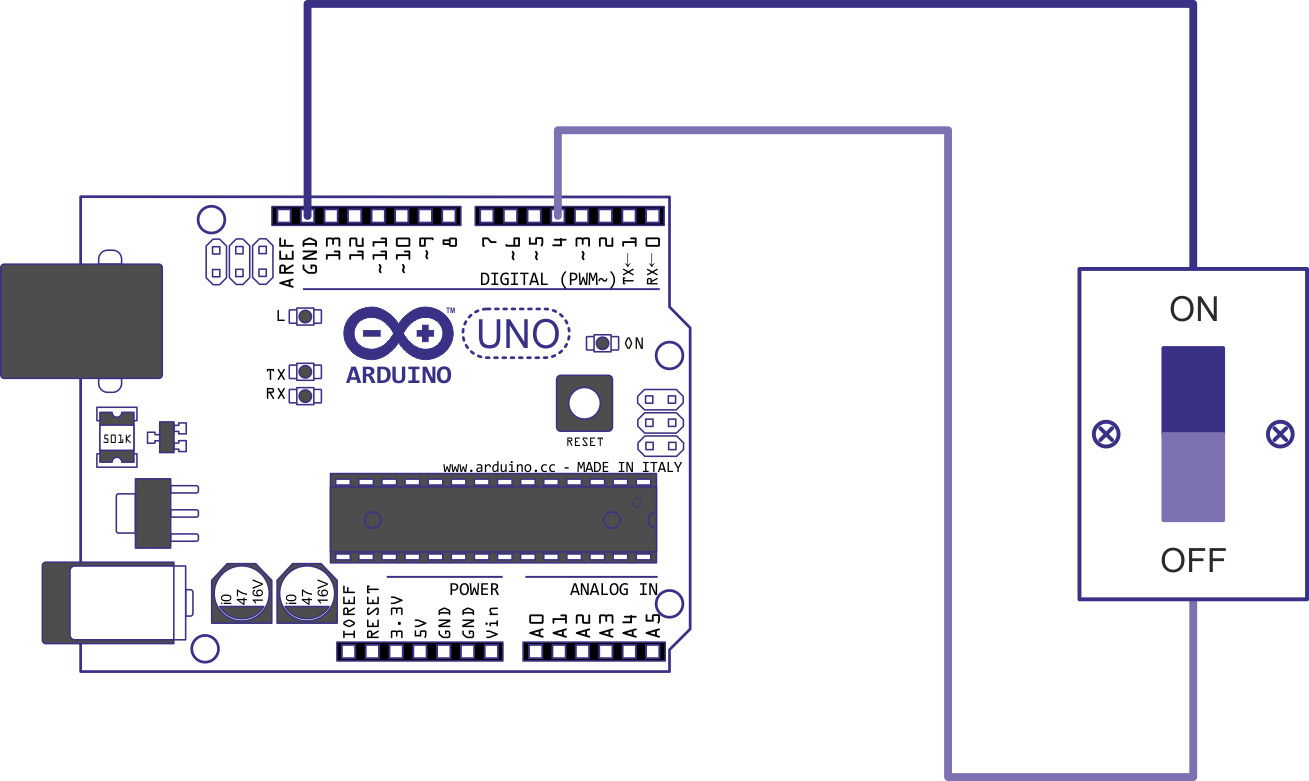
\includegraphics[width=0.8\textwidth]{imagenes/arduino_interruptor.png}
     \caption{Ejemplo de conexión Arduino y un interruptor}
     \label{fig:conexion-ard-int}
    \end{figure}
 
 
 El segundo cambio a introducir es posibilitar el accionado de las luminarias de manera digital, es decir, controlado desde el nodo. Para esto utilizaremos el circuito de la figura \ref{fig:circuito_int}. 
 
\begin{figure}[htb]
    \centering
    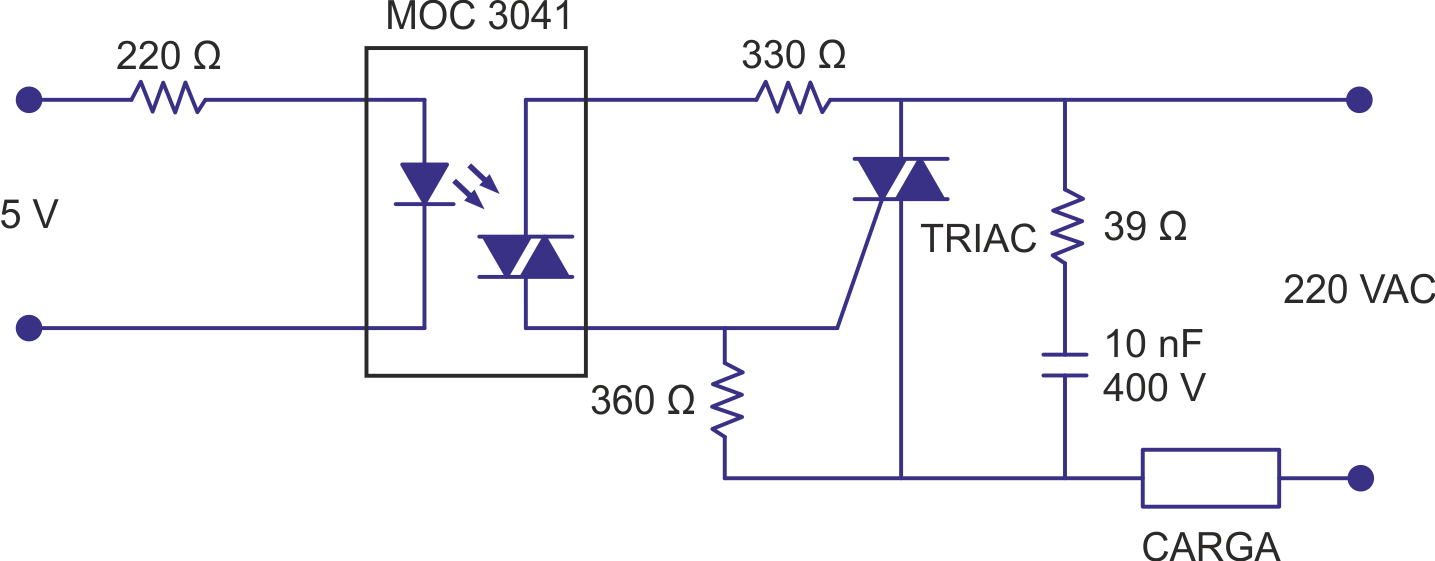
\includegraphics[width=0.8\textwidth]{imagenes/circuito_interruptor.png}
    \caption{Circuito interruptor}
    \label{fig:circuito_int}
\end{figure}
 
 Este circuito, conocido como relé de estado sólido, nos permite accionar cualquier carga eléctrica desde el nodo. Su funcionamiento es muy sencillo: el nodo activa el led dentro del optoacoplador, este hace que el triac del optoacoplador empiece a conducir, lo cual activa el triac principal, que es el que maneja realmente la carga. 
 
 Hemos elegido como optoacoplador el MOC3041 porque incorpora <<detección de paso por cero>>. El optoacoplador espera a que la señal de  alterna pase por cero para abrir o cerrar el paso de corriente. Gracias a este comportamiento se reduce el estrés en los aparatos, ya que la señal eléctrica les llega gradualmente, y se consigue una vida útil mas larga.
  
En la figura \ref{fig:ard_int_lamp} se muestra esquema de conexión entre un nodo, el relé y una lampara.

\begin{figure}[htb]
    \centering
    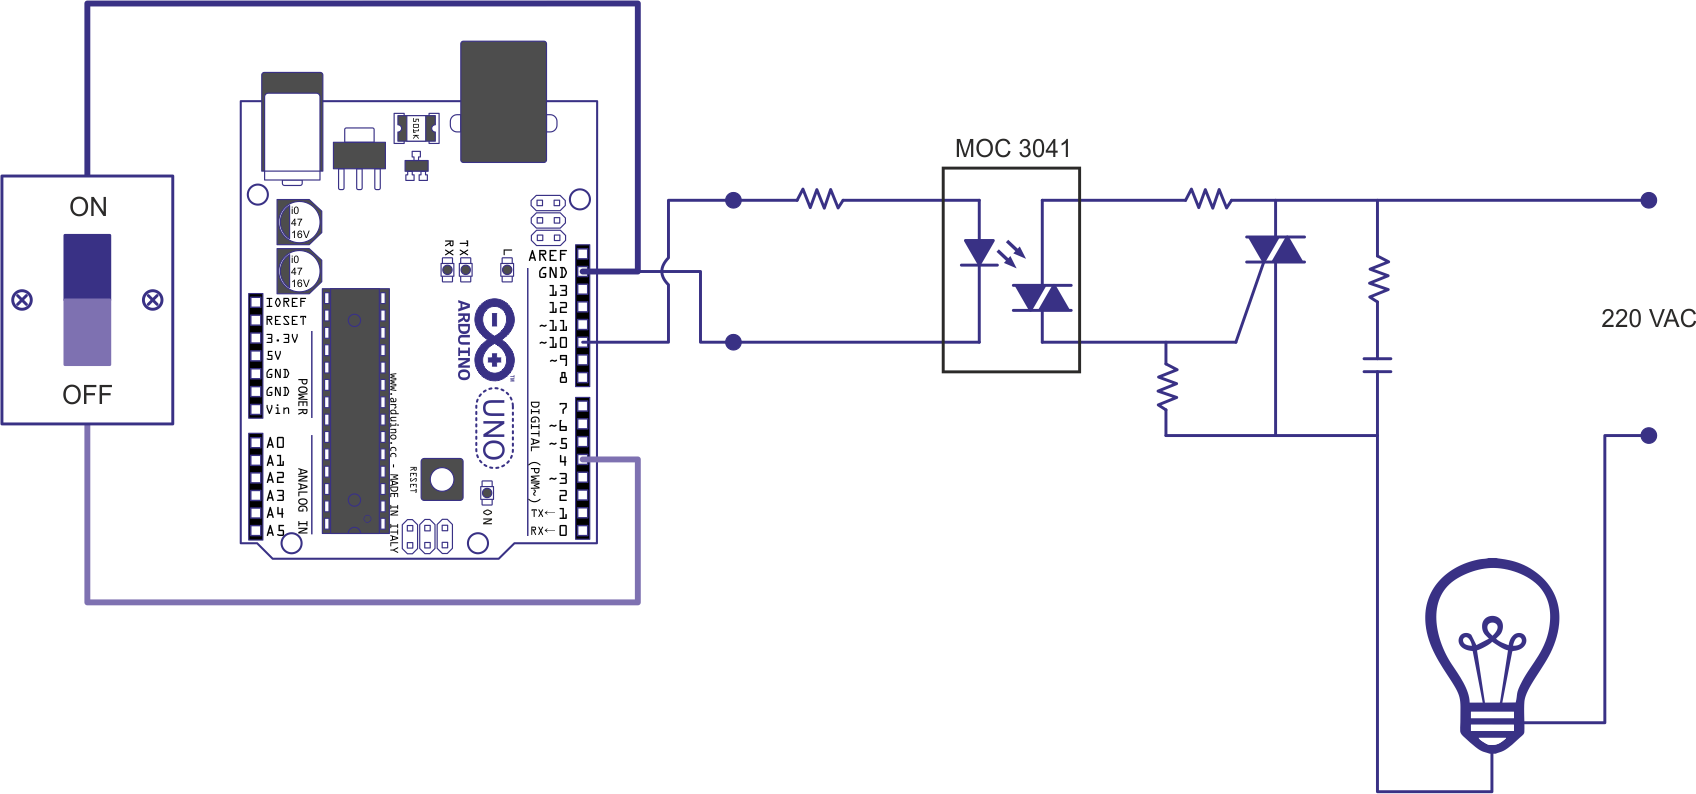
\includegraphics[width=0.8\textwidth]{imagenes/arduino_lampara.png}
    \caption{Ejemplo de conexión: Arduino, interruptor, relé y lámpara}
    \label{fig:ard_int_lamp}
\end{figure}

Cada Arduino dispone de 14 pines de entrada/salida digitales, estos son los que utilizaremos para conectar los interruptores y actuadores(relés). Los pines analógicos los reservaremos para conectar los sensores.

\subsection{Funcionamiento}

El código que se ejecuta en cada Arduino consta de tres partes: <<configuración>>, <<setup>>, <<loop>>.
\subsubsection{Configuración}
En esta parte del código es donde se configuran todos los parámetros que necesita Arduino para funcionar.

Lo primero es definir la identificación del nodo.
\begin{lstlisting}

const char MY[] = "01";

\end{lstlisting}

Después, tenemos que especificar en que patillas están conectados los interruptores, los actuadores, y la relación de ambos.

\begin{lstlisting}

#define NUM_INT 1
int PIN_INTERRUPTORES[NUM_INT] = {7};


int INTERRUPTOR_ACTUADOR[NUM_INT] = {0};


#define NUM_ACT 2
int PIN_ACTUADORES[NUM_ACT] = {11, 13};

\end{lstlisting}

En el array <<INTERRUPTOR\_ACTUADOR>> es donde se relacionan los interruptores con los actuadores. La posición dentro del array hace referencia al interruptor, y el valor de dicha posición referencia al actuador correspondiente En el ejemplo mostrado, el primer interruptor esta conectado al pin 7 de Arduino, y el actuador que debe accionarse es el de la posición 0, es decir, el actuador en el pin 11.

Acto seguido se configuran los pines de los sensores, temperatura, movimiento y luz. Ademas de la posición (dentro del vector <<PIN\_ACTUADORES>>) del actuador del sensor de movimiento, y el tiempo que éste debe estar encendido en milisegundos. 

\begin{lstlisting}{breaklines=true}

int PIN_TEMPERATURA = 1;
int ARRAY_TEMPERATURA[10];


int PIN_PIR = 10;
int ACTUADOR_PIR = 0;
int TIEMPO_PIR = 3000;


int PIN_LDR = 2;
\end{lstlisting}

El resto del código hasta la siguiente sección, son variables globales necesarias para el correcto desarrollo de Arduino. Aquí no es necesaria la configuración.

\begin{lstlisting}

// Vector de estado de interruptores

int ESTADO_INTERRUPTORES[NUM_INT];


// Vector de valores de los actuadores


int VALOR_ACTUADORES[NUM_ACT];


// Variables de control de mensajes


int FUNCION_MSJ, ACTUADOR_MSJ, VALOR_MSJ;


// Flags


int FLAG_PIR = 0;
int FLAG_MSJ = 0;

// Timers


unsigned long TIMER_INTERRUPTOR[NUM_INT];
unsigned long TIMER_PIR;

\end{lstlisting}

El array <<ESTADO\_INTERRUPTORES>> se usa para monitorizar el valor de cada interruptor, en busca de cambios entre lo almacenado y el actual, para detectar pulsaciones del usuario.

En el array <<VALOR\_ACTUADORES>> se almacena el valor de todos los actuadores.

Las variables: <<FUNCION\_MSJ>>, <<ACTUADOR\_MSJ>>, <<VALOR\_MSJ>>, se usan en las tareas de descodificación de los mensajes recibidos de la red.

Las <<flags>> se utilizan para comunicar eventos dentro del programa.

Por último tenemos los <<timers>> o temporizadores, éstos se utilizan para evitar el uso de sentencias como \lstinline[]|delay()|. En ellos se almacena el tiempo que Arduino lleva encendido, función \lstinline|millis()|, y en sucesivas vueltas del <<loop>> se comprueba el tiempo que ha pasado.


\subsubsection{Setup}
Esta parte del código solo se ejecuta una vez, justo al encenderse el Arduino.

Aquí usamos la información introducida en la <<configuración>> para ajustar los parámetros internos del microcontrolador e inicializar las comunicaciones. El código es el siguiente:

\begin{lstlisting}
void setup() {
    Serial.begin(9600);
    int i;
    
    //Interruptores, inicializacion
    for(i = 0; i < NUM_INT; i++){
        pinMode (PIN_INTERRUPTORES[i], INPUT_PULLUP);
        ESTADO_INTERRUPTORES[i] = 
           digitalRead (PIN_INTERRUPTORES[i]);
    TIMER_INTERRUPTOR[i] = 0;
    }
    
    //Actuadores, inicializacion
    for(i = 0; i < NUM_ACT; i++){
        pinMode(PIN_ACTUADORES[i], OUTPUT);
        VALOR_ACTUADORES[i] == 0;
    }
    
    //Sensores
    pinMode(PIN_PIR, INPUT);
}
\end{lstlisting}

Empieza por configurar el puerto serie a 9600 baudios. 

Luego, se configuran los pines correspondientes a los interruptores como entradas, y se activan las resistencias <<pull-up>> internas del microcontrolador. La razón de usar las resistencias internas es eliminar circuitería extra de cara al usuario.

También se configuran los pines de los actuadores como salidas digitales, y los pines de los sensores como entradas.

A la vez que se configuran los pines, se inicializan los valores de los vectores <<ESTADO\_INTERRUPTORES>> Y <<VALOR\_ACTUADORES>>.

\subsubsection{Loop}
Como ya sabemos el <<loop>> es un bucle que se ejecuta sin parar y hasta el infinito dentro de Arduino. Aquí es donde reside toda la lógica del nodo.

Lo hemos dividido en varias secciones, que se ejecutan en orden.

\begin{enumerate}
    \item Recepción de mensajes.
    \item Sensores e Interruptores.
    \item Actualización de actuadores.
\end{enumerate}

\subsubsection{Recepción de mensajes}
En esta parte, cada vez que se inicia de nuevo el <<loop>>, miramos si hemos recibido algo por el puerto serie. Si esto es así, llamamos a la función \lstinline|recibeMensaje()|, donde esperamos a terminar de recibir el mensaje, se descodifica y activamos la bandera de recepción de mensaje.

\begin{lstlisting}
if(Serial.available() > 0){
    recibeMensaje();
    if(FLAG_MSJ == 1){
        FLAG_MSJ = 0;
        procesaMensaje();
    }
}
\end{lstlisting}

Acto seguido, se procesa el mensaje, ejecutando la orden recibida.

\subsubsection{Sensores e interruptores}
Esta sección se subdivide en otras dos partes: control de interruptores y lectura de sensores.

Veamos primero el control de los interruptores. El código:
\begin{lstlisting}
for(i = 0; i < NUM_INT; i++){
    est_aux = digitalRead(PIN_INTERRUPTORES[i]);

    if(est_aux != ESTADO_INTERRUPTORES[i]){
        ESTADO_INTERRUPTORES[i] = est_aux;

        if(TIMER_INTERRUPTOR[i] == 0){
            TIMER_INTERRUPTOR[i] = millis();
            cambiaActuador(INTERRUPTOR_ACTUADOR[i]);
        }
    }

    if(TIMER_INTERRUPTOR[i] != 0 && 
            (millis() - TIMER_INTERRUPTOR[i] > 1000)){
        TIMER_INTERRUPTOR[i] = 0;
    }
}
\end{lstlisting}


Como vimos anteriormente, en el escenario sobre el que trabajamos lo que tenemos son interruptores convencionales. Por ello, para controlarlos, buscamos cambios en el estado; es decir, saltos tanto de 0 a 5V como de 5 a 0V. 

Teniendo lo anterior en cuenta, el proceso es el siguiente: se recorre el array de interruptores, <<PIN\_INTERRUPTORES>>, comprobando el estado que tenemos guardado con el actual. En caso de encontrar algún cambio, guardamos el nuevo estado, activamos el timer correspondiente y llamamos a la función \lstinline|cambiaActuador()|. Esta función lo único que hace es guardar en el array <<VALOR\_ACTUADORES>> el nuevo valor, para su posterior actualización y notifica a la Raspberry el nuevo valor del actuador.


Si se ha detectado un cambio, pero el timer aun sigue activo, solo guardamos el nuevo estado para las siguientes comprobaciones. Al cabo de 1000 milisegundos, desactivamos el timer y vuelve a empezar el ciclo.

Lo siguiente en el <<loop>> es leer el valor de los sensores. Esto lo hacemos leyendo el sensor y guardando los valores sobre un array de 10 posiciones de forma cíclica. Luego, cuando se solicite el valor de alguno de los sensores, se realiza una media aritmética de los valores del array, así, se obtienen lecturas más estables.

\begin{lstlisting}
ARRAY_TEMPERATURA[bucle_sensor] = 
         analogRead(PIN_TEMPERATURA);
//Luz
array_luz[bucle_sensor] = analogRead(PIN_LDR);


bucle_sensor = (bucle_sensor + 1) % 10;
\end{lstlisting}


Lo siguiente y último de esta parte es el control del sensor de movimiento. 

Para activar la luz del sensor de movimiento lo primer es comprobar que la bandera del sensor no este activa. Esta bandera se activa al encenderse la luz de forma explícita, sin que el sensor se active. Además, por supuesto, tiene que activarse el sensor.

Una vez el sensor se ha activado, comprobamos la cantidad de luz que hay en la habitación, ya que es posible que no haga falta encender nada. Si todo está bien, se ha activado el sensor y no hay luz suficiente, se activa el temporizador del sensor y se actualiza el valor en el array de actuadores.

En el caso de que se active el sensor, y el temporizador ya este activo, nos saltamos la comprobación de la luz, puesto si el temporizador esta activo significa que la luz esta encendida y por lo tanto esta comprobación siempre dará negativo, por que hay luz. En este caso solo reiniciamos el temporizador.

Una vez ha pasado el tiempo configurado por el usuario, desactivamos el temporizador y apagamos la luz.

El código para esto es el siguiente:

\begin{lstlisting}
if(FLAG_PIR == 0 && digitalRead(PIN_PIR) == HIGH){

    if(TIMER_PIR == 0){
        for(i = 0; i < 10; i++){
            cantidad_luz += array_luz[i];
        }
        cantidad_luz = cantidad_luz / 10;
    }else{
        cantidad_luz = 0;
    }

    if(cantidad_luz < 500){
        TIMER_PIR = millis();
        VALOR_ACTUADORES[ACTUADOR_PIR] = 1;
    }
}


if( TIMER_PIR != 0 
   && (millis() - TIMER_PIR > TIEMPO_PIR)){
        TIMER_PIR = 0;
        VALOR_ACTUADORES[ACTUADOR_PIR] = 0;
}
\end{lstlisting}


\subsubsection{Actualización de actuadores}
Por último se actualizan los actuadores a los valores nuevos. En el array <<VALOR\_ACTUADORES>> tenemos almacenado el valor que deben tener los actuadores, así, recorremos el array escribiendo por la salida de cada actuador su valor correspondiente. 




\begin{lstlisting}

for(i = 0; i < NUM_ACT; i++){
    if(VALOR_ACTUADORES[i] == 0){
        digitalWrite(PIN_ACTUADORES[i], LOW);
    }else{
        digitalWrite(PIN_ACTUADORES[i], HIGH);
    }
}

\end{lstlisting}

Antes de terminar, hay que destacar una característica de los nodos: el funcionamiento tanto de los interruptores físicos, como del sensor de movimiento, están programados completamente dentro de Arduino. Esto quiere decir que cada uno de los nodos es completamente autónomo en el funcionamiento más básico. Aunque, por ejemplo, el router o la Raspberry no estén operativos, o se caiga la red XBee; el funcionamiento físico nunca se perderá.

\section{Estación base - Raspberry Pi}
La estación base, o la Raspberry Pi en nuestro sistema, es la encargada de gestionar todo el sistema. Desde aquí se gestionan las conexiones y se ejecutan las tareas de alto nivel.

\subsection{Ubicación}
A priori, lo ideal sería ubicar la Raspberry cerca del router doméstico, pues se supone que será un punto cercano al centro de la vivienda, y ademas se podría conectarla a el directamente con un cable Ethernet. Aunque esto no pueda ser así, tampoco es un problema ya que la conexión con la red de sensores es inalámbrica, y existe la posibilidad de añadir un dongle Wi-Fi para la conexión a la red doméstica.

\subsection{Equipamiento}

El equipamiento adicional necesario para la Raspberry solo consta de dos elementos, el resto lo trae de serie.

El primer elemento que hay que añadirle es un módulo XBee. Para ello existen en el mercado diversas opciones, como por ejemplo el módulo <<XBee Xplorer>> este permite conectar una placa XBee a un puerto USB de la Raspberry. En la fotografía de la figura \ref{fig:foto_xbeexplorer} podemos ver uno. Lo importante, más allá del producto o método utilizado, es que la conexión con el módulo XBee sea a través del puerto serie.

\begin{figure}[htbp]
    \centering
    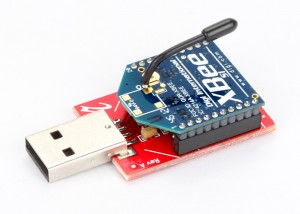
\includegraphics[width=0.80\textwidth]{imagenes/xbeexplorer.jpg}
    \caption{Módulo XBee Explorer}
    \label{fig:foto_xbeexplorer}
\end{figure}

El segundo elemento es para proporcionar conectividad con la red doméstica, esto puede ser un simple cable Ethernet, o un dongle Wi-Fi, es indiferente.


\subsection{Estructura lógica}

El funcionamiento lógico de la Raspberry está dividido en tres bloques. 

Una base de datos, que nos proporciona una estructura en la que almacenar la información necesaria para la gestión del sistema. 


Un servidor central, donde se procesan las peticiones de la aplicación de usuario y los mensajes de la red, se envían las órdenes pertinentes y se actualiza la información de la base de datos.

Por último, la aplicación de usuario, en ésta se proporciona una interfaz gráfica para el manejo del sistema. Desde ella se activan y desactivan las luces y las escenas, se programan las acciones, etc... Además, sirve para configurar el sistema a través de la base de datos.

\subsection{Base de datos}
\begin{figure}[htbp]
    \centering
    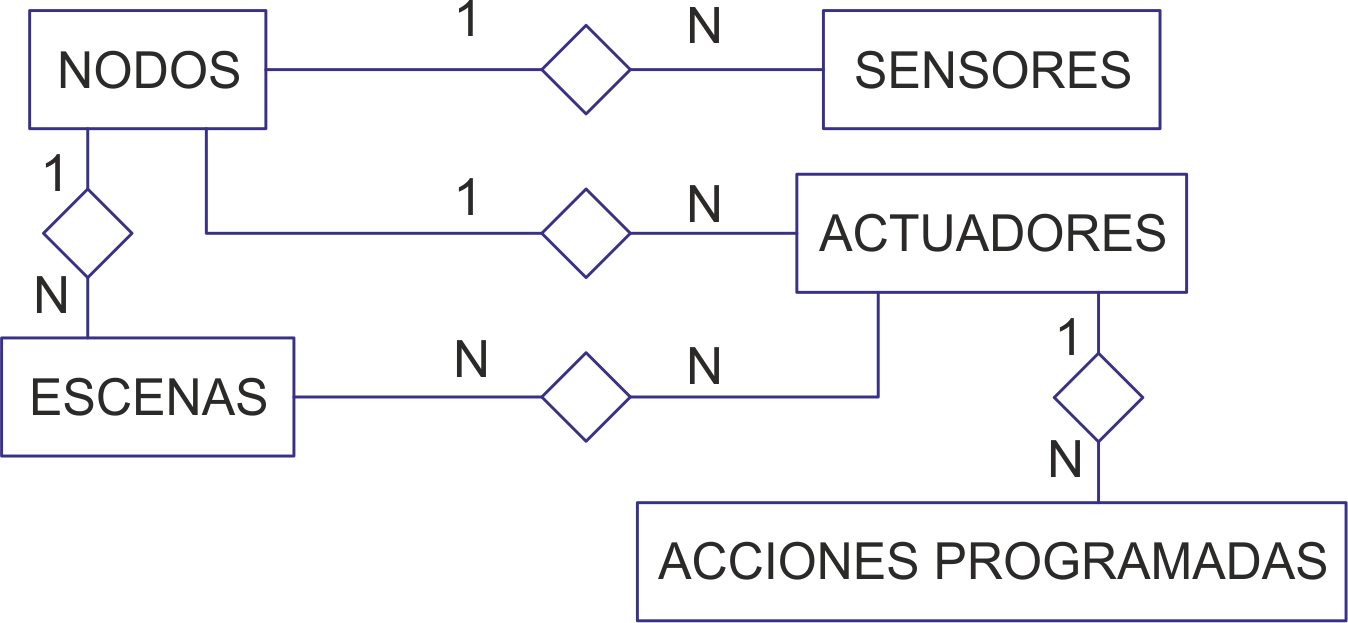
\includegraphics[width=0.80\textwidth]{imagenes/esquema_bd.png}
    \caption{Esquema de la base de datos}
    \label{fig:esquema_bd}
\end{figure}

El esquema lo podemos ver en la figura \ref{fig:esquema_bd}. La base de datos se ha diseñado para cumplir con los requisitos actuales, y que sea fácilmente ampliable en un futuro.



Las entidades que hemos considerado relevantes son:
\begin{description}
    \item[Nodos] Esta entidad hace referencia, indistintamente, a los arduinos que componen la red de sensores, y a las habitaciones donde se encuentran. Se almacenan los datos relativos a estos.
    \item[Sensores] Aquí se almacena todo lo relativo a los sensores monitorizados de los nodos. En nuestro caso, solo tenemos sensores de temperatura. 
    \item[Actuadores] Esta entidad modela las luminarias instaladas en cada nodo. 
    \item[Escenas] Éstas son las distintas configuraciones fijas de una habitación, que por alguna razón el usuario considere guardar.
    \item[Acciones programadas] En esta entidad se modela las órdenes de encendido o apagado a alguna hora determinada.
\end{description}

Estas entidades, y sus relaciones, se traducen en el siguiente conjunto de tablas.

\begin{itemize}
   \item Nodos \{id, my, estancia\}
   \item Sensores\{id, tipo\_sensor, valor, nodo\_id\}
   \item Actuadores\{id, nombre, posicion, estado, nodo\_id\}
   \item Escenas\{id, nombre, nodo\_id\}
   \item Actuador\_Escena\{escena\_id, actuador\_id, estado\}
   \item Acciones\{id, nombre, estado, actuador\_id\}
   \item Accion\_dia\{accion\_id, dia\_sem\}
\end{itemize}





\subsection{Servidor central}

 Desde el punto de vista del software, si consideramos la programación de los nodos como la capa de nivel mas bajo, y la aplicación de usuario como la de nivel mas alto, el servidor central ocupa la capa intermedia. Actúa como puente de unión o nexo entre ellas.
 
 El servidor se ha escrito desde cero, y el lenguaje elegido es Python, en su última versión. 
 
 La estructura del servidor está dividida en tres hilos: uno para la interfaz con la red de sensores, otro para la interfaz con la aplicación, y un tercero para gestionar el sistema. 
 
 
 Para las comunicaciones internas del servidor usamos varios objetos del tipo <<Queue>>. Estos objetos son un tipo de cola que permiten el paso de información entre hilos de forma eficiente, ya que trae implementado de serie los mecanismos de seguridad y control necesarios.
 
 El funcionamiento a grandes rasgos es el siguiente. 
 
 El hilo <<interfaz wsn>> esta constantemente esperando a recibir o un mensaje de la red, que lo pasa al hilo de gestión; o a recibir un mensaje para enviar a la red, que inmediatamente después de recibirlo lo envía a través del puerto serie.
 
 El hilo <<interfaz app>> está esperando una conexión desde la aplicación de usuario, cuando la recibe, extrae la petición y se la envía al hilo de gestión.
 
 En el hilo de gestión, se procesan los mensajes de la red para actualizar la base de datos, se traducen las peticiones en mensajes para la red, y se ejecutan tareas periódicas como pedir la temperatura de las habitaciones y se establecen las alarmas para las acciones programadas.
 
 El script principal es el siguiente:
 \begin{lstlisting}
 if __name__ == "__main__":
     recibidos = queue.Queue()
     a_enviar =  queue.Queue()
     peticiones = queue.Queue()
 
     hilopcm =
        pcm.Pcm(recibidos, a_enviar, peticiones)
     hilopcm.start()
 
     hilowsn = 
       interfazwsn.InterfazWsn(recibidos, a_enviar)
     hilowsn.start()
 
     hiloapp = 
       interfazapp.InterfazApp(a_enviar, peticiones)
     hiloapp.start()
 \end{lstlisting}
 
 En este script se crean los tres objetos <<Queue>> que necesitamos.
 \begin{description}
     \item[recibidos] En esta cola se almacenan los mensajes recibidos desde la red de sensores.
     \item[a\_enviar] Aquí se almacenan los mensajes salientes hacia la red.
     \item[peticiones] En esta cola guardamos las peticiones que van llegando desde la aplicación de usuario.
    \end{description}
 
 A continuación se crean los tres hilos que manejan el sistema y se les pasan las colas que necesitan cada uno. Al <<hilowsn>>, <<recibidos>> y <<a\_enviar>>; al <<hiloapp>>, solo <<peticiones>>; y al <<hilopcm>>, las tres colas. Una vez creados se inicia su ejecución con la función \lstinline|Threading.start()|.
 
 \subsubsection{Hilo interfaz red de sensores}
 
 Este script se encarga de envolver las comunicaciones con la red de sensores. Para ello, se inicializa el puerto serie, y se monitoriza constantemente tanto el puerto serie, como la cola de envíos. 
 
 El script es el siguiente:
  \begin{lstlisting}
  class InterfazWsn(threading.Thread):
      def __init__(self, rec, env):
          threading.Thread.__init__(self)
          self.recibidos = rec
          self.enviar = env
      
      def run(self):
          wsn = serial.Serial("/dev/ttyACM0", 
                      baudrate=9600, timeout=1.0)
          while True:
              if wsn.inWaiting() > 0:
                  msj_b = wsn.readline()
                  msj = msj_b.decode('ascii')
                  self.recibidos.put(msj)
          
              if self.enviar.qsize() > 0 :
                  msj = self.enviar.get()
                  self.enviar.task_done()
                  msj_b = msj.encode()
                  wsn.write(msj_b)
  \end{lstlisting}
 
 
 Cuando recibe un mensaje desde la red, este está en formato <<byte>>, binario, así que lo decodifica en <<ascii>>(función \lstinline|msj_b.decode('ascii')|), y lo envía al hilo de gestión, \lstinline|recibidos.put(msj)|.
 
  Al recibir un mensaje a enviar, hace el proceso inverso. Lo convierte en formato <<byte>>, función \lstinline|msj.encode()|, lo envía por el puerto serie, \lstinline|wsn.write(msj_b)|.
  
  
 \subsubsection{Hilo interfaz aplicación de usuario}
 
 Para este hilo hemos creado un pequeño servidor <<TCP>>. Este servidor, también basado en hilos, escucha por el puerto <<TCP 9999>> a la espera de comunicaciones de la aplicación de usuario. Cuando una de éstas llega, crea un hilo nuevo para esa conexión y vuelve a la espera.
 
 En el hilo nuevo, la aplicación comunica su petición a través de un objeto <<JSON>>. Si éste es correcto, se pasa inmediatamente al hilo de gestión y se envía un <<ok>> de vuelta a la aplicación. En caso de no ser un <<JSON>> correcto, se obvia la petición y se manda hacia atrás un <<fail>>.
 
 El script es el siguiente:
 \begin{lstlisting}
 class InterfazApp(threading.Thread):
     def __init__(self, pet):
         threading.Thread.__init__(self)
         self.peticiones = pet
         self.a_enviar = envio
 
     def run(self):
         servidor = socket.socket(socket.AF_INET,
                  socket.SOCK_STREAM)
         servidor.setsockopt(socket.SOL_SOCKET, 
                 socket.SO_REUSEADDR, 1)
         servidor.bind(('localhost', 9999))
         servidor.listen(5)
         i = 0
         while True:
             conn, (host, puerto) = servidor.accept()
             handler = AppHandler(conn, host, puerto, 
                     self.a_enviar, self.peticiones)
             handler.start()
         servidor.close()
 \end{lstlisting}
 
 En esta primera parte, se crea el hilo con las colas correspondientes, el socket tcp, y se pone a la escucha del puerto, \lstinline|servidor.accept()|. Cuando entra una conexión, crea el objeto que la manejará, \lstinline|AppHandler(...)|, y lo inicia.
 
 La clase que maneja la información que transmite la aplicación es la siguiente:
 \begin{lstlisting}
 class AppHandler(threading.Thread):
     def __init__(self,con, host, puerto, envia, pet):
         threading.Thread.__init__(self)
         self.conexion = con
         self.peticiones = pet
         self.host = host
         self.puerto = puerto
         self.a_enviar = envia
 
     def run(self):
         data  = self.conexion.recv(1024)
         data = data.decode('UTF-8')
         deco  = json.loads(data)
         respuesta = ""
 
         if ('peticion' in deco):
             self.peticiones.put(deco)
             respuesta = '{ ok : 1 }'
             else:
             respuesta = '{ fail : 0 }'
 
 
         response = json.dumps(respuesta)
 
         self.conexion.send(bytes(response, 'utf8'))
 
         self.conexion.close()
 \end{lstlisting}
 
Una vez creado el objeto, recibe los datos, los descodifica en  <<JSON>>, y se comprueba que exista el campo <<peticion>>. Si esto es así, encola la petición, \lstinline|peticiones.put(deco)|, crea el <<ok>> de respuesta y lo envía, y cierra la conexión. Si el <<JSON>> no contuviera el campo <<peticion>>, significa que no es una petición válida, por lo que creará una respuesta <<fail>> y la enviará. 

El motivo de realizar las comunicaciones entre el servidor en Python y la aplicación de usuario a través de conexiones <<TCP>> es flexibilizar el sistema. De esta manera, se puede descentralizar la aplicación y ésta podría estar ejecutandose en otra máquina. O por ejemplo, crear una aplicación específica para un sistema operativo, y que ésta siga teniendo acceso al sistema. Además, los objetos <<JSON>> son casi un estándar de facto en las comunicaciones entre aplicaciones, con lo que, crear estas aplicaciones alternativas no debería ser un problema.


\subsubsection{Hilo de gestión}

En este hilo es donde reside la mayor parte de la lógica del servidor. El script está dividido estructuralmente en tres partes: tratamiento de mensajes de la red, tratamiento de peticiones de la aplicación y acciones periódicas.

El script se inicia con el constructor de la clase. En éste se crean las variable para albergar las colas de comunicación, se abre la conexión con la base de datos, y por último se crea el array que contendrá los objetos <<Timer>>.

\begin{lstlisting}
class Pcm(threading.Thread):
    def __init__(self, rec, env, pet):
        threading.Thread.__init__(self)
        self.recibidos = rec
        self.enviar = env
        self.peticiones = pet
        self.bd = pymysql.connect(host='127.0.0.1', 
                                  port=3306,
                                  user='root', 
                                  passwd='xxxxx', 
                                  db='platymo')
        self.timers = []
\end{lstlisting}

El objeto <<Timer>> es un objeto especial de la clase <<Threading>>, la clase encargada de los hilos de ejecución en Python. Al constructor de este objeto se le pasa una cantidad de tiempo, en segundos, y una función. Al cabo ese tiempo ejecuta la función y se destruye. En nuestro sistema, éstos objetos se utilizan para programar envíos de mensajes en diferido, las acciones programadas del sistema. 

El código para el procesado de los mensajes de la red es el siguiente:
\begin{lstlisting}
if self.recibidos.qsize() > 0 :
    msj = self.recibidos.get()
    self.recibidos.task_done()

    my = msj[:2]
    func = msj[2:4]
    act = msj[4:6]
    val = msj[6:9]

    if func == "10":
        self.setValBDActuador(my, act, val)
    elif func == "20":
        self.setValBDSensor(my, act, val)
    elif func == "00":
        self.setApagarTodo(my)
\end{lstlisting}

Cuando se recibe un mensaje, se descodifica y dependiendo de su contenido se aplica una función u otra. 

\begin{description}
    \item[setValBDActuador(my, act, val)] Actualiza el valor del actuador en la base de datos.
    \item[setValBDSensor(my, act, val)] Actualiza el valor del sensor en la base de datos.
    \item[setApagarTodo(my)] Actualiza todos los actuadores del nodo en cuestión al valor 0.
\end{description}


Para el procesamiento de las peticiones de la aplicación, el método a seguir es análogo al anterior.
\begin{lstlisting}
if self.peticiones.qsize() > 0:
    peticion = self.peticiones.get()
    self.peticiones.task_done()

    if peticion['peticion'] == "actuador":
        self.setActuador(peticion['id'],
                     peticion['valor'])
    elif peticion['peticion'] == "escena":
        self.activarEscena(peticion['escena'])
    elif peticion['peticion'] == "apagarTodo":
        self.apagarTodo()
    elif peticion['peticion'] == "actualizarTimers":
        self.setTimers()
\end{lstlisting}
 
 \begin{description}
     \item[ setActuador(peticion('id'), peticion('valor')) ] Envía a la red el mensaje correspondiente para activar o desactivar el actuador.
     \item[activarEscena(peticion('escena'))] Esta función accede a la configuración de la escena, guardada en la base de datos, y envía los mensajes correspondientes.
     \item[apagarTodo()] Envía el mensaje <<000000000>>, que activa el apagado de todos los actuadores en todos los nodos.
     \item[setTimers()] Esta función busca en la base de datos todas las acciones programadas para el día actual, y posteriores a la hora actual. Con esta información crea los objetos <<Timer>> necesarios.  A esta función se la llama cada vez que una <<acción programada>> es creada o modificada en la aplicación.
    \end{description}
    
    
 La última parte del script realizamos todas las gestiones dependientes del tiempo. Éstas son: cada 5 minutos actualizar el valor de los sensores de temperatura y  a las 00:00 de cada día crear los <<Timers>> correspondientes.
 
 El código:
 \begin{lstlisting}
 fechahora = time.localtime()
 minmodulo = fechahora[4] % 10
 
 if (minmodulo == 0 or minmodulo == 5):
     if flag_temperatura:
         self.peticionTemperatura()
         flag_temperatura = False
     else:
         flag_temperatura = True
 
 if (fechahora[3] == 0 and fechahora[4] == 0):
     if flag_timers:
         self.setTimers()
         flag_timers = False
     else:
         flag_timers = True
 \end{lstlisting}
    
  La secuencia es la siguiente: guardamos la hora actual, y si los minutos acaban en 0 o 5 simplemente se pide a todos los nodos de la red que reporten el valor del sensor de temperatura. Cuando los mensajes de respuesta de éstos lleguen, la parte del código de tratamiento de mensajes es la encargada de guardar la información.
  
  Después, comprobamos si son las 00:00, en caso afirmativo, llamamos a la función \lstinline|setTimers()| para crear los <<Timers>> correspondientes y dejar el sistema listo para el día que empieza.
  
  Las variables <<flag\_timers>> y <<flag\_temperatura>> se utilizan para que el script ejecute una sola vez las órdenes dentro del minuto correspondiente.
  
  
  \subsection{Aplicación de usuario}
  
  La aplicación de usuario es la última capa de software. Actúa como interfaz para el manejo diario del sistema y como método de configuración. Se ha escrito como una aplicación web para que el acceso sea mas universal, así, se puede acceder a ella desde ordenadores personales, teléfonos inteligentes, o tabletas.
  
  Como se ha podido observar, desde el servidor en Python solo se accede a la base de datos para extraer o actualizar información. Es desde la aplicación desde donde se inicializa o se introduce información nueva. Para el usuario final es más sencillo, y además está más acostumbrado, tratar con formularios web que, por ejemplo,  con la linea de comandos o programas específicos para bases de datos.
  
  La aplicación está escrita en PHP, concretamente usando el framework Laravel. Éste framework implementa el patrón MVC, lo que nos da una estructura, tanto de archivos como lógica, ya definida.
  
  En Laravel todo empieza con las <<rutas>>, éstas son unas URLs, definidas previamente, que se encargan de dirigir la aplicación a un controlador u otro. En los controladores se prepara la información, accediendo a los modelos de la base de datos tanto para crear nuevos, como para actualizarlos. Después, esta información se pasa a las vistas, que es lo que ve el usuario.
  
  Para las vistas, usaremos también un framework, Bootstrap, esto nos ofrece dos grandes ventajas principalmente:
  \begin{enumerate}
      \item Bootstrap incluye un sistema de rejilla para la disposición de los elementos, completamente enfocado al diseño responsable. Esto propicia que la aplicación se muestre correctamente sea cual sea el tamaño de la pantalla.
      \item También incluye una serie de elementos de interfaz definidos y listos para usar, con lo que el desarrollo es más rápido, y nos asegura un aspecto uniforme en toda la aplicación.
    \end{enumerate}
    
 En resumen, necesitamos crear: los modelos de la base de datos,  los controladores, las vistas y definir las rutas de cada pantalla de la aplicación.
 
 Conceptualmente, la aplicación se divide en dos partes: la zona de configuración, donde se crean y editan los distintos elementos del sistema, y la zona principal, donde se encienden y apagan los actuadores, se activan las escenas, en definitiva, el manejo diario.
 
 Lo primero que veamos serán los modelos, puesto que son de uso común en toda la aplicación.
 
 
 \subsubsection{Modelos}
 
 Si recordamos el esquema de la base de datos, figura \ref{fig:esquema_bd}, se ha creado un modelo por cada una de las entidades. Estos son:
 \begin{itemize}
     \item Nodo
     \item Actuador
     \item Sensor
     \item Escena
     \item Accion
    \end{itemize}
    
    Como ejemplo de la implementación de los modelos, veamos el código del modelo del nodo.
    
    \begin{lstlisting}
    class Nodo extends Model {
    
        protected $table = 'nodos';
    
        public function sensores(){
            return $this->hasMany('App\Sensor');
        }
    
        public function actuadores(){
            return $this->hasMany('App\Actuador');
        }
    
        public function escenas(){
            return $this->hasMany('App\Escena');
        }
    }
    \end{lstlisting}
    
    Primero se establece que tabla de la base de datos contiene al modelo. El ORM de Laravel automáticamente hace accesible todos los campos que contenga la tabla, solo hay que decirle las relaciones que existen con los demás modelos. Para esto, se crean las funciones que siguen.
    
    En este caso, como todas las relaciones del nodo son <<uno a varios>>, se utiliza la función \lstinline|hasMany('Modelo')|. Esta función es la que establece la relación <<uno a varios>> dentro del ORM.
    
    Para establecer la relación inversa, en el modelo del actuador, por ejemplo, se debe crear otro método, esta vez hay que utilizar \lstinline|belongsTo('Modelo')|. El código sería:
    \begin{lstlisting}
    class Actuador extends Model {
    
        protected $table = 'actuadores';
        
        public function nodo(){
            return $this->belongsTo('App\Nodo');
        }
        
        public function acciones(){
            return $this->hasMany('App\Accion');
        }
        
        public function escenas(){
            return $this->belongsToMany('App\Escena');
        }
    }
    \end{lstlisting}
    
    A partir de este momento, desde cada objeto <<Nodo>> se podrá acceder a los sensores, actuadores y escenas asociados, y  a la inversa.
    
    El resto de modelos siguen la misma estructura.
    
    \subsubsection{Zona principal}
    
    Esta zona es el punto de entrada del usuario. 
    
    La primera pantalla, <<panel principal>>, da acceso a todas las demás partes de la aplicación. Su aspecto se puede ver en la figura \ref{fig:panel_ppal}
    
    \begin{figure}[htbp]
        \centering
        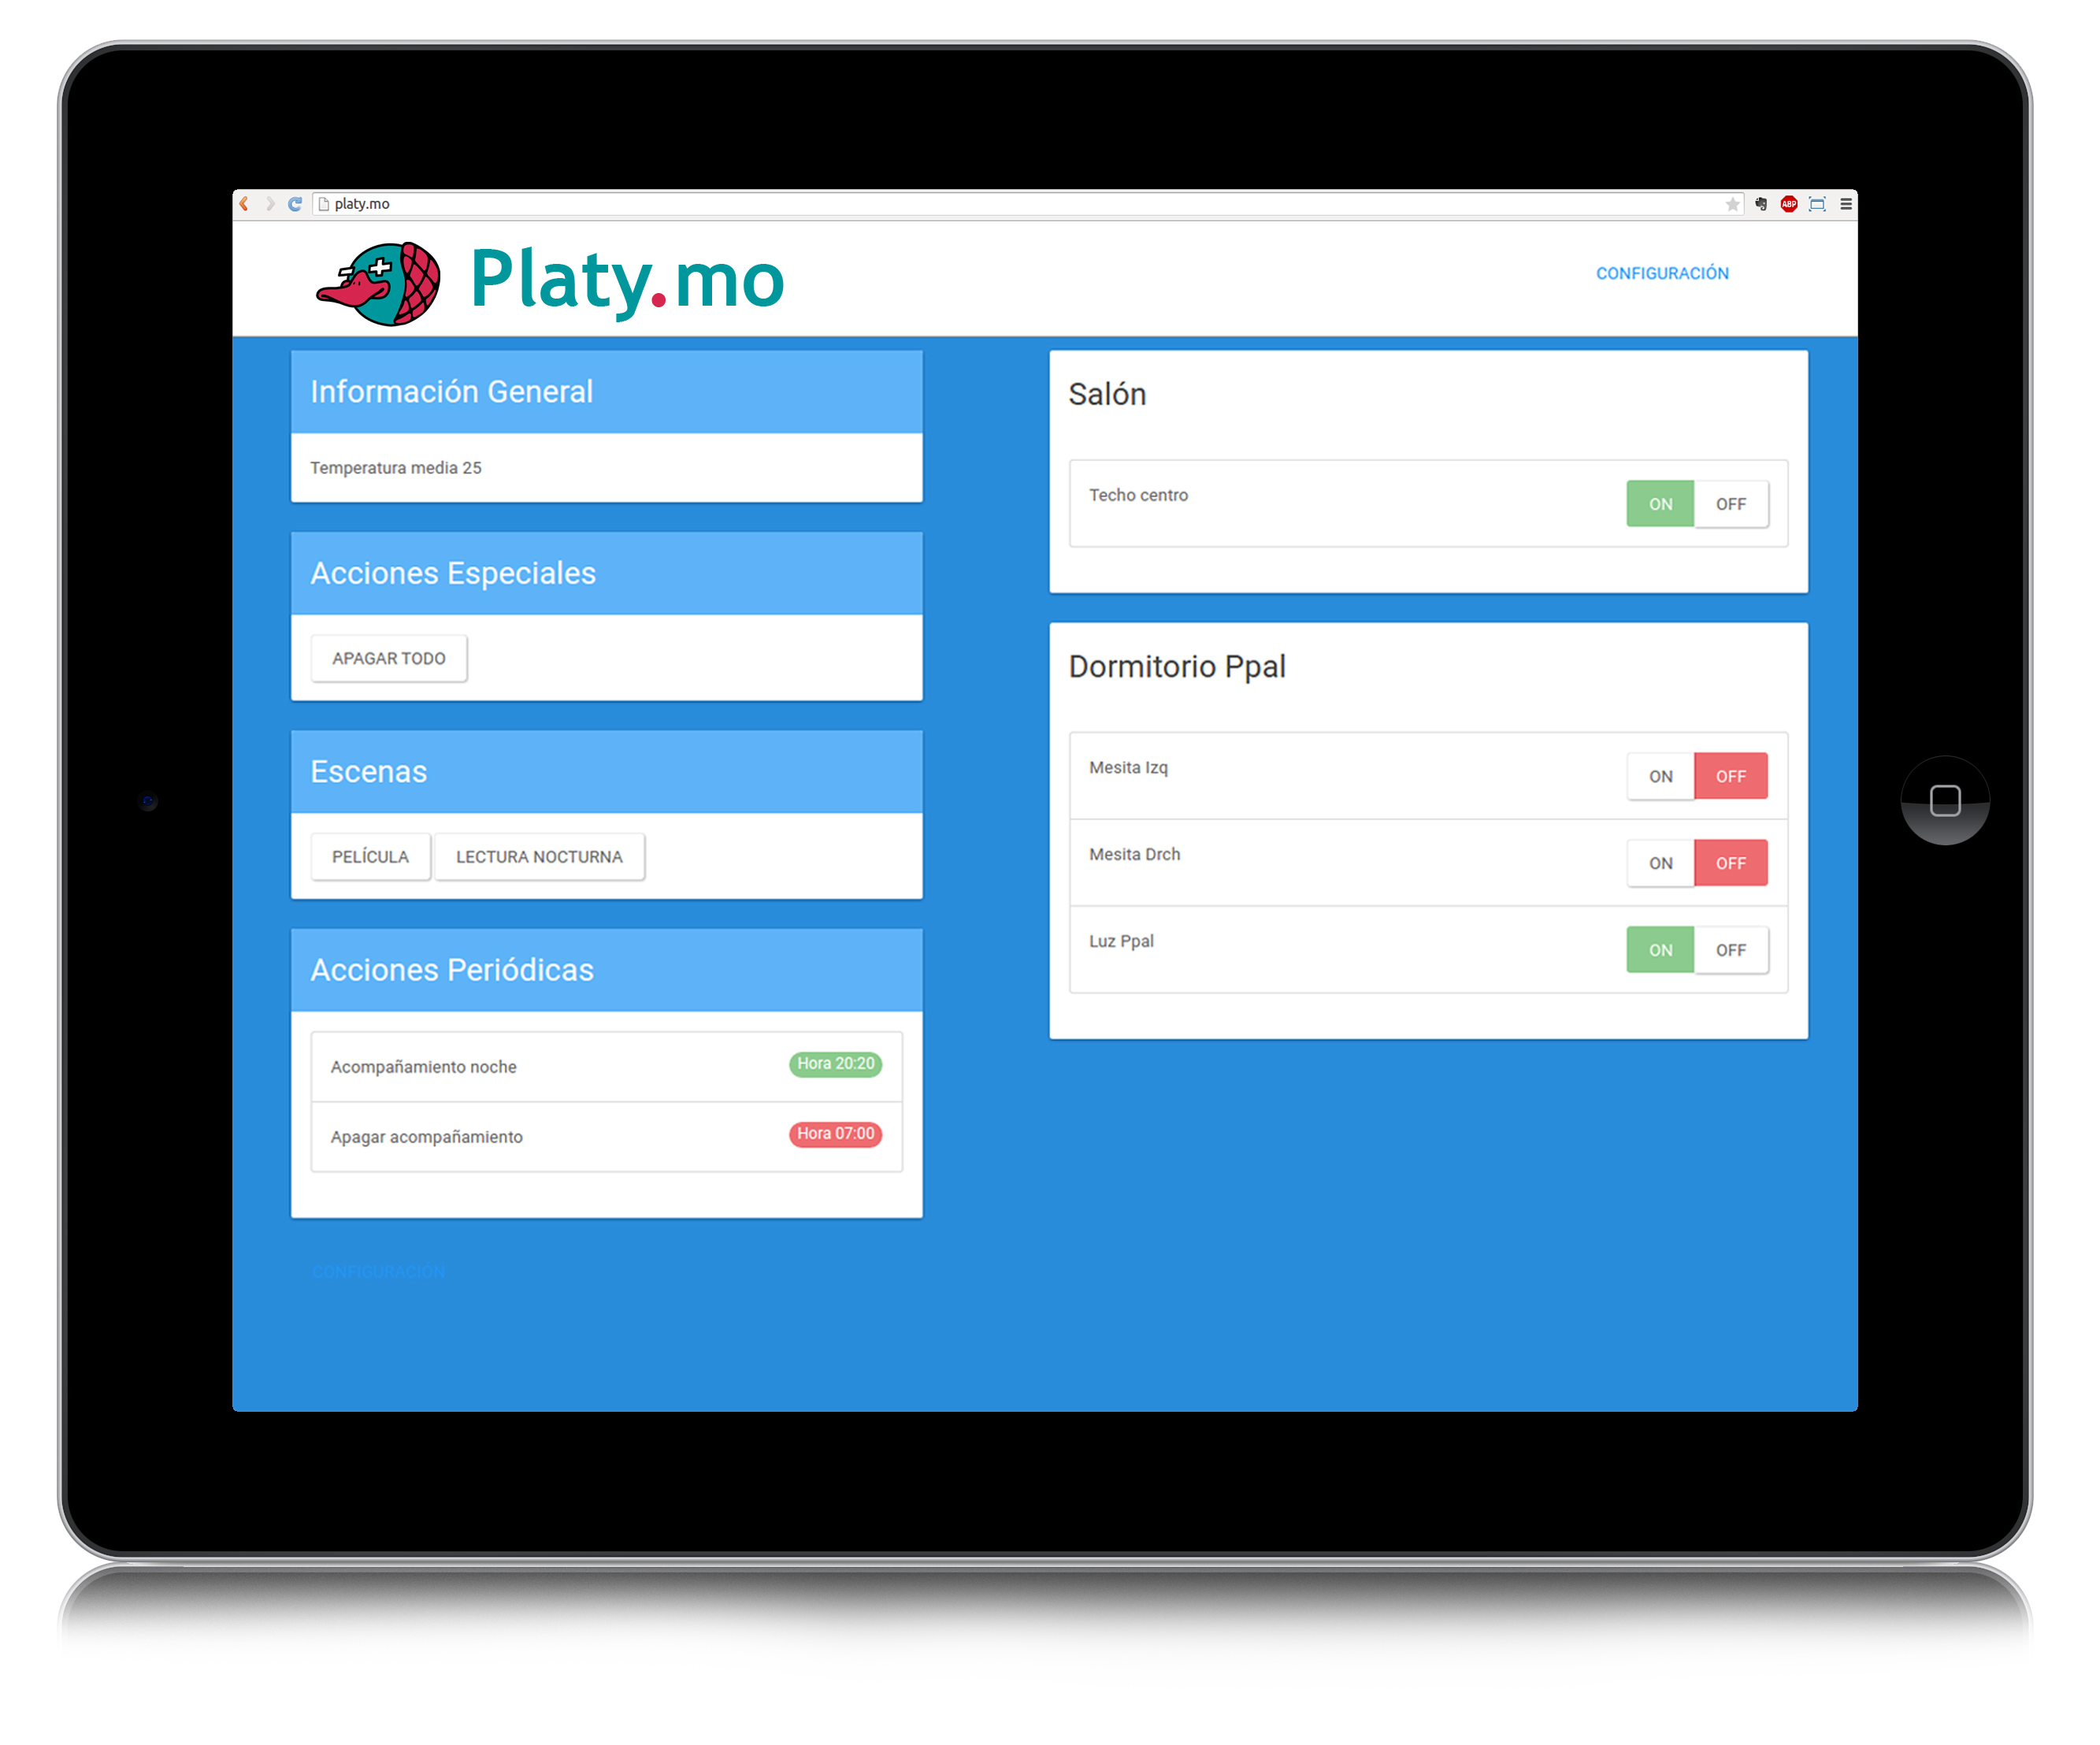
\includegraphics[width=0.95\textwidth]{imagenes/panel_ppal.jpg}
        \caption{Panel principal}
        \label{fig:panel_ppal}
    \end{figure}
    
    Esta pantalla esta dividida en dos columnas.
    
     A la izquierda, información general, acceso a las funciones especiales y las escenas, y una lista con todas las acciones programadas que existan. En la lista de las acciones programadas, el color de fondo donde se muestra la hora indica si se enciende o se apaga, verde y rojo respectivamente. Tanto las funciones especiales, como las escenas son botones para activarlas.
     
     A la derecha, tenemos un panel para cada habitación, en este panel se pueden accionar algunas luminarias de la habitación, estos botones también sirven como indicadores de su estado actual. Y, si pulsamos en la parte superior del panel, nos llevará a la vista detallada de la habitación. 
    
    En la esquina superior derecha, encontramos el enlace hacia la configuración. De esta zona hablaremos mas adelante.
    
   Toda esta zona esta gestionada por un único controlador, <<PrincipalController>>. En éste, se definen tres métodos: \lstinline|home()|,  \lstinline|vista()|, \lstinline|configuracion()|. Cada uno de ellos da paso a: el panel principal, la vista detallada de las habitaciones, y el panel de configuración, respectivamente. Para la zona en la que estamos, solo nos fijaremos en las dos primeras.
    
    Las rutas que definen esta parte son:
    \begin{lstlisting}
    Route::get('/', 'PrincipalController@home');
    Route::get('vista/{id}', 
                'PrincipalController@vista');
    \end{lstlisting}
    
    Como podemos observar, la ruta <</>> activa el método \lstinline|home()| que nos renderiza la pantalla que acabamos de ver. Su código:
    \begin{lstlisting}
    public function home(){
    
        $habitaciones = Nodo::all();
        $array_panel = array();
        $i = 0;
        
        foreach ($habitaciones as $habitacion) {
          $array_panel[$i] = array();
          $array_panel[$i]['habitacion']=$habitacion;
          $array_panel[$i]['actuadores'] = array();
          $j = 0;
          foreach ($habitacion->actuadores()
                    ->where('principal', 1)->get()
                             as $act) {
                    
            $array_panel[$i]['actuadores'][$j] = $act;
            $j++;
        }
            $i++;
        }
        
        $escenas = Escena::all();
        $acciones = Accion::all();
        
        
        
        return view('home.principal')->
                   with(array('panel' => $array_panel,
                              'escenas' => $escenas,
                              'acciones' => $acciones,
                              'title' => ''));
    }
    \end{lstlisting}
    
    En el código, primero se prepara toda la información necesaria, y después, retorna la vista correspondiente añadiéndole la información recavada.
    
    De forma análoga a la anterior, la función \lstinline|vista($id)|, muestra la pantalla <<vista detallada>>, figura \ref{fig:vista_hab}; cuando se accede a la ruta <</vista/{id}>>, siendo \{id\} una variable que contiene el id de la habitación o nodo. Hay que destacar, que esta variable es extraída de la URL.
    
     \begin{figure}[htbp]
         \centering
         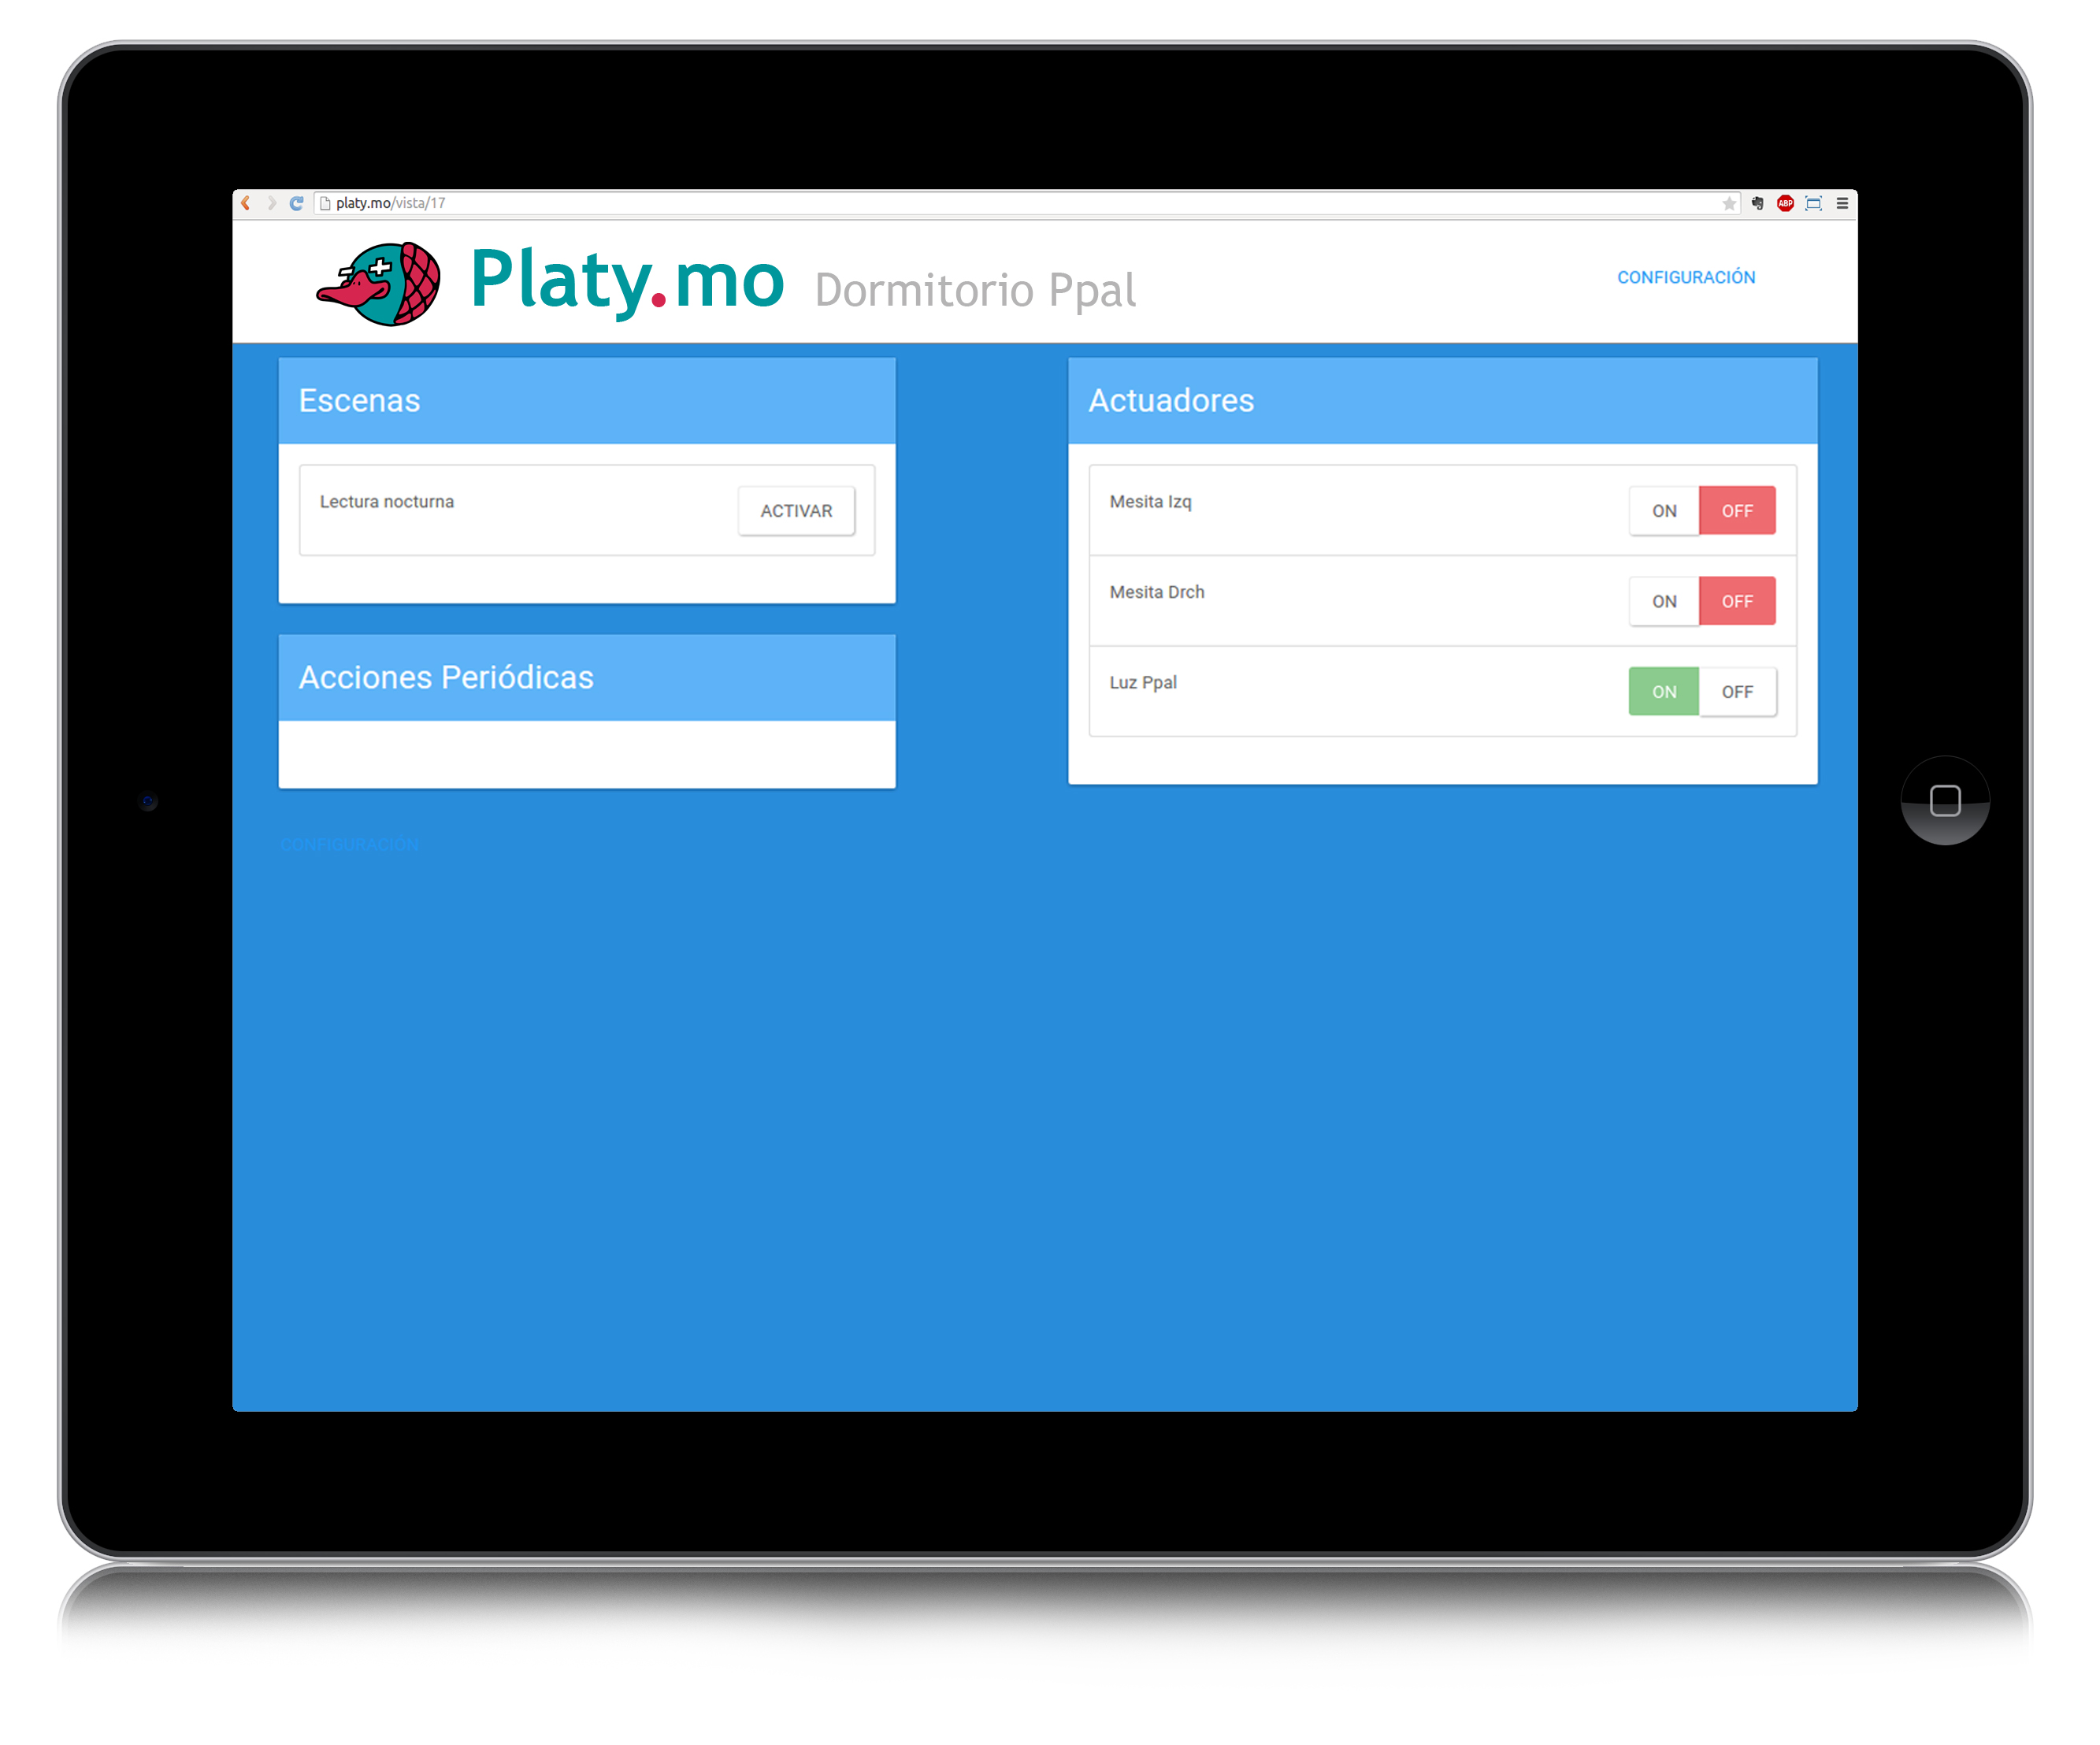
\includegraphics[width=0.95\textwidth]{imagenes/vista.jpg}
         \caption{Vista detallada de las habitaciones}
         \label{fig:vista_hab}
        \end{figure}
        
        
    En esta pantalla podemos ver toda la información relativa a la  habitación: las escenas y acciones configuradas y la lista completa de luminarias instaladas. 
    
    Cuando pulsamos en algún botón para activar algo, tanto en el panel principal como en las habitaciones, realmente lo que hacemos es pulsar sobre un enlace. Este enlace nos lleva a un controlador creado explícitamente para enviar las peticiones al servidor en Python, <<ComandoController>>
    
    Las rutas definidas para <<ComandoController>> son:
    \begin{lstlisting}
    Route::get('comando/actuador/{id}/{valor}',
                        'ComandoController@actuador');
                 
                 
                 
    Route::get('comando/escena/{id}',
                         'ComandoController@escena');
                 
    Route::get('comando/apagar', 
                      'ComandoController@apagarTodo');
    \end{lstlisting}
    
    Tomemos como ejemplo <</comando/actuador/\{4\}/\{0\}>>, en esta ruta pondríamos el actuador con id igual a 4, a valor 0, es decir, apagar el actuador 4. Para ello, la función \lstinline|actuador($id, $valor)| de <<ComandoController>> hace lo siguiente.
    
    \begin{lstlisting}
    public function actuador($id, $valor){
        $datos = array();
    
        $actuador = Actuador::find($id);
    
    
        $datos['peticion'] = 'actuador';
    
        $datos['id'] = $actuador->id;
        $datos['valor'] = (int)$valor;
    
        PythonComm::envia($datos);
    
    
        return redirect()->back();
    }
    \end{lstlisting}
    
    Se crea un array de claves con los valores: <<petición>>, actuador; <<id>>, id del actuador, <<valor>>, el valor deseado. En nuestro ejemplo quedaría como muestra la tabla \ref{tab:pet_ejem}.
    
    \begin{table}[h]
        \centering
        \begin{tabular}{c|c}
            \toprule
            peticion & actuador  \\ 
            id & 4       \\ 
            valor & 0    \\\bottomrule
        \end{tabular}
        \caption{Petición de ejemplo}
        \label{tab:pet_ejem}
    \end{table}
    
    Una vez montado el array, se llama a la función \lstinline|envia($datos)| de la librería <<PythonComm>>. Esta librería, se encarga de enviar datos hacia el servidor Python. Una vez enviados los datos, se redirecciona al usuario hacia la pantalla desde la que activara el botón, \lstinline|redirect()->back()|.
    
    En la función \lstinline|envia($datos)|, simplemente se abre un socket, el array <<\$datos>> se codifica en <<JSON>>, se envían por el socket, y se cierra la conexión. 
    
    El resto de las funciones de <<ComandoController>> funcionan de la misma forma, solo que cambiando los datos de la petición.
    
   
    \subsubsection{Zona de configuración}
    
    La zona de configuración esta construida como una serie de formularios web, a los que se accede desde un panel principal. Se accede a través de la ruta <</configuracion>>, que activa el método \lstinline|configuracion()| del <<PrincipalController>>. El proceso es el mismo, se preparan los datos necesarios, y se renderiza la vista, figura \ref{fig:panel_config}.
    
     \begin{figure}[htbp]
         \centering
         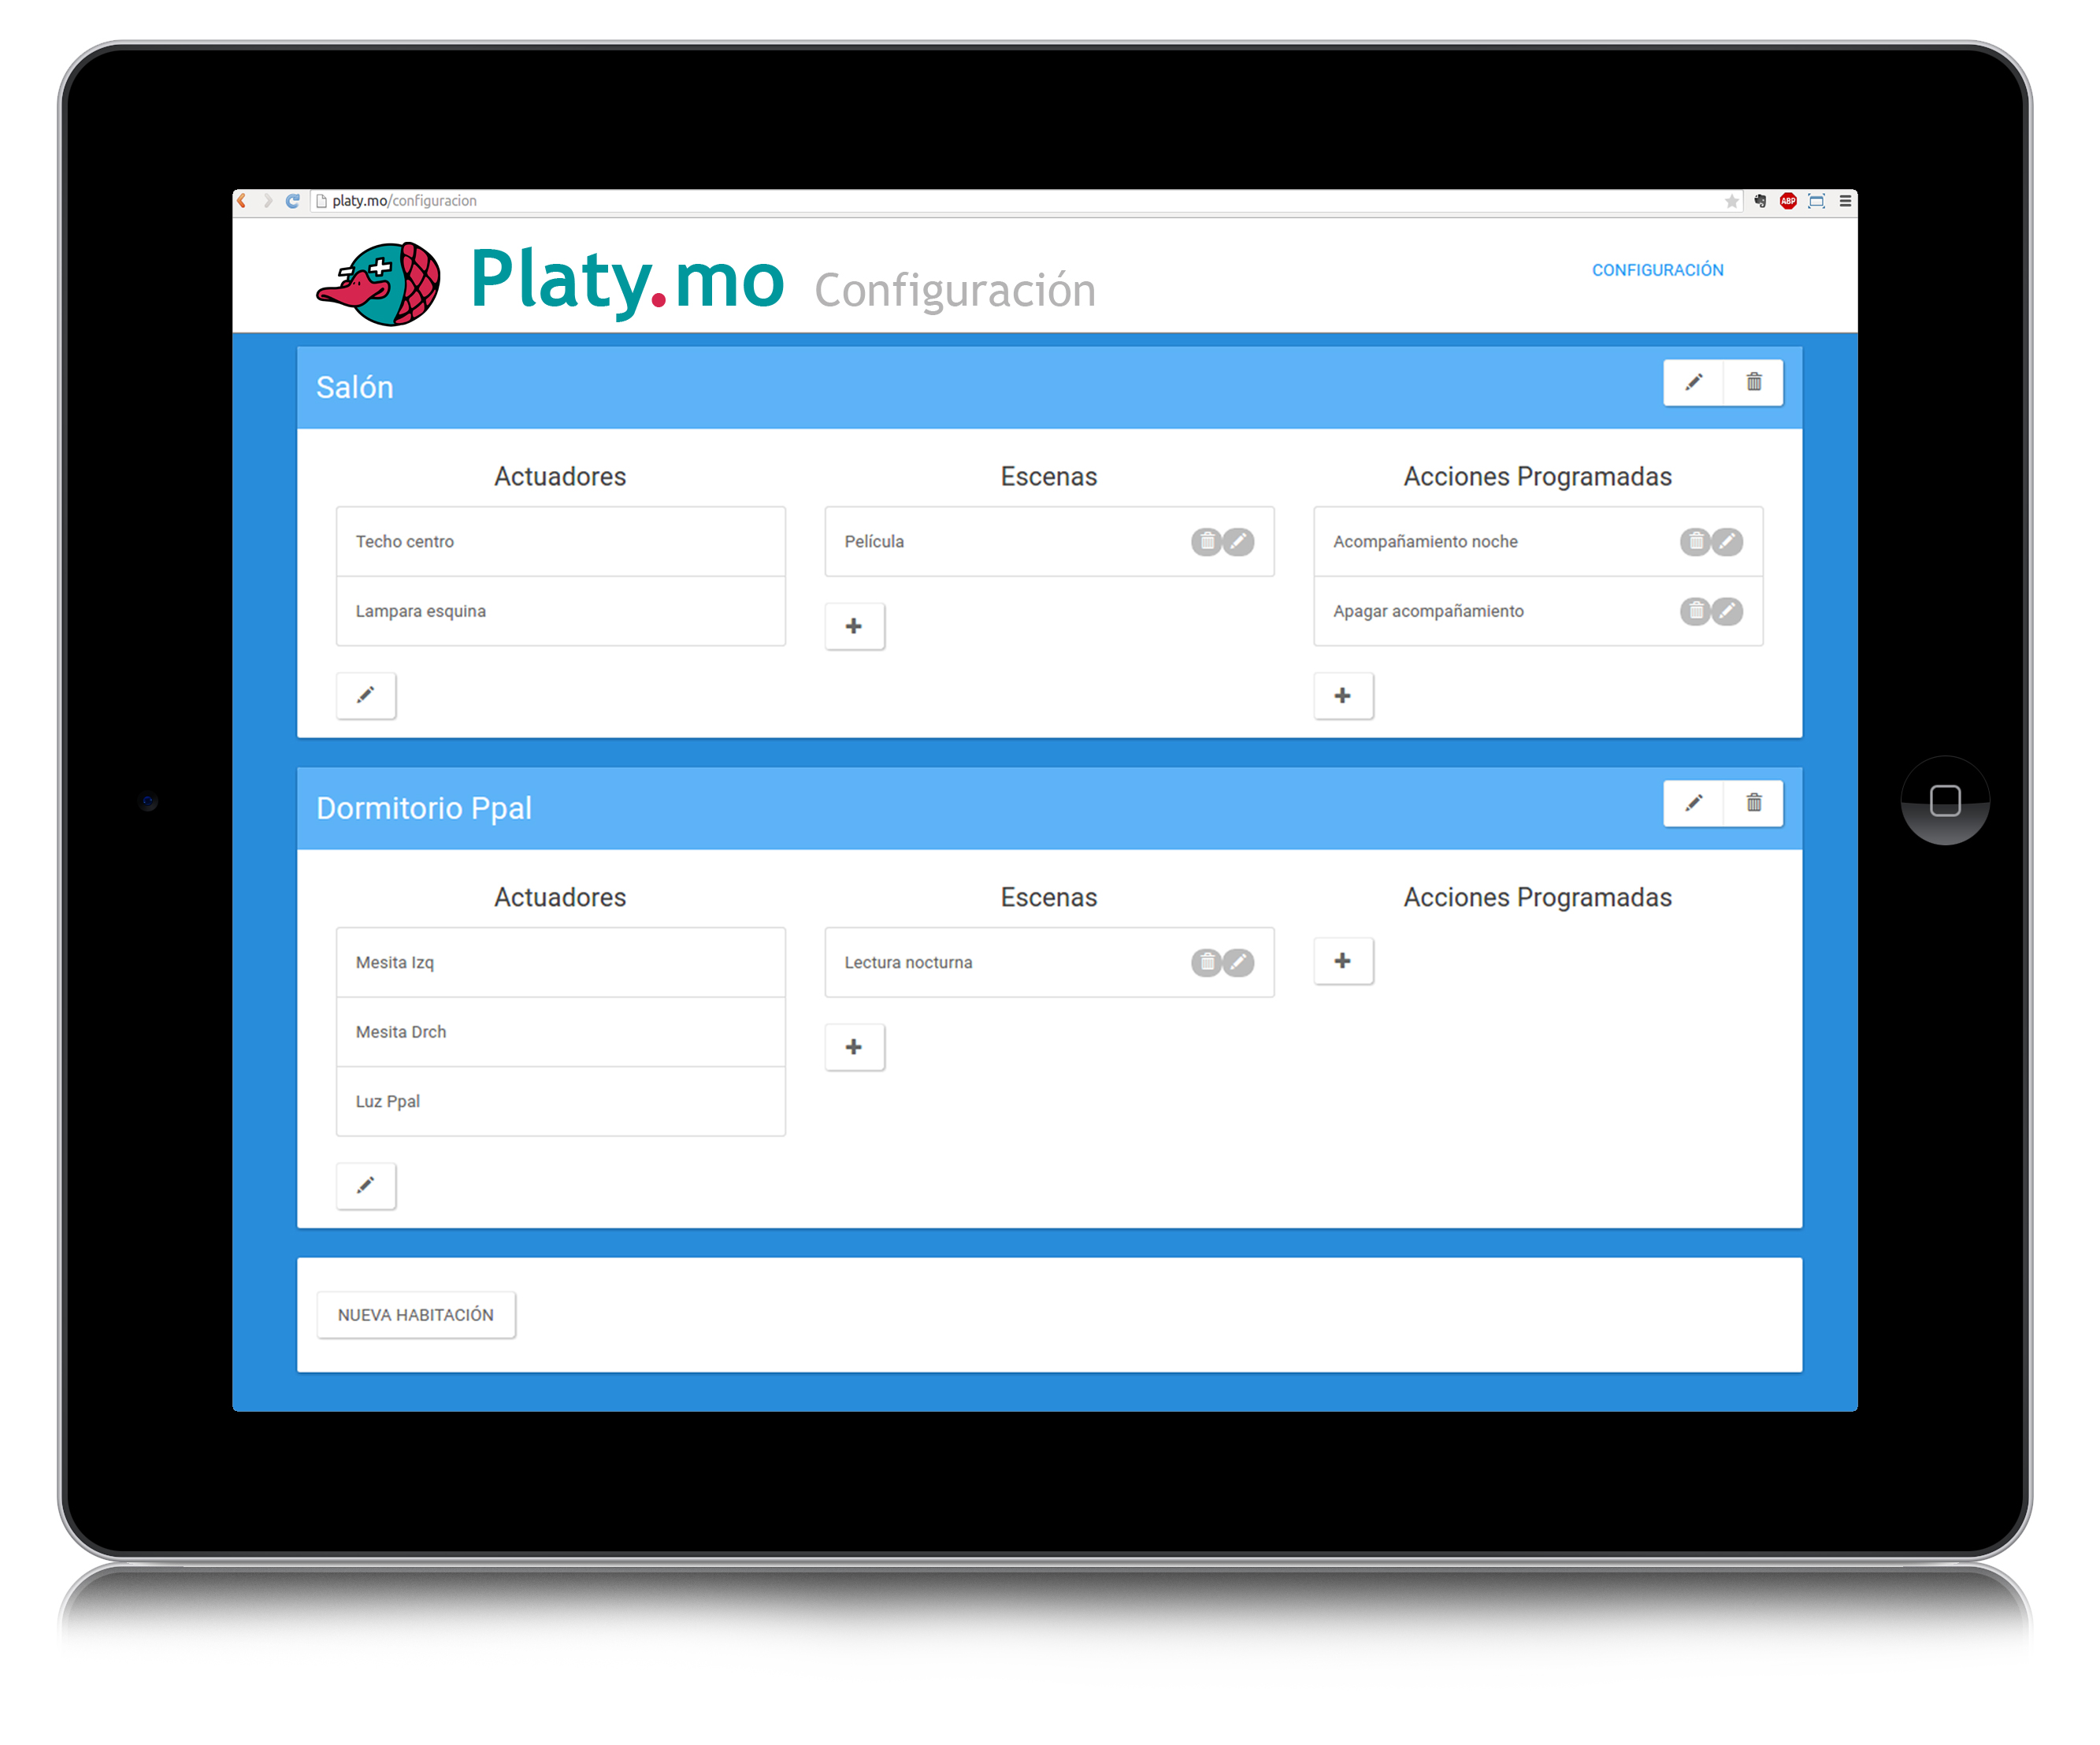
\includegraphics[width=0.95\textwidth]{imagenes/panel_config.jpg}
         \caption{Panel de configuración}
         \label{fig:panel_config}
        \end{figure}
        
    Este panel se organiza en función de las habitaciones que existan en el sistema. Una tarjeta para cada una de ellas. Estas tarjetas, se dividen en tres partes: lista de actuadores o luminarias, lista de escenas, y lista de acciones programadas.
    
    Como se puede observar en la captura de pantalla, cada panel habitación tiene dos botones en la parte superior derecha, para editar o borrar la habitación al completo. Abajo del todo de la pantalla, encontramos el botón <<Nueva Habitación>>, con él, creamos una nueva habitación. 
    
    Cada escena y cada acción tienen dos botones a su derecha, borrado y edición. El botón <<+>> creará una escena o acción nueva según el que pulsemos.
    
    El formulario para añadir o editar una habitación, es el que se muestra en la figura \ref{fig:form_hab}. En él introduciremos tanto la información de la habitación, <<my>> del nodo, y el nombre de ésta, como los actuadores correspondientes, su nombre, la posición dentro del array <<PIN\_ACTUADORES>>en el código del Arduino, y si queremos que se muestre en el panel principal o no.
    
    
    
        \begin{figure}[h!]
            \centering
            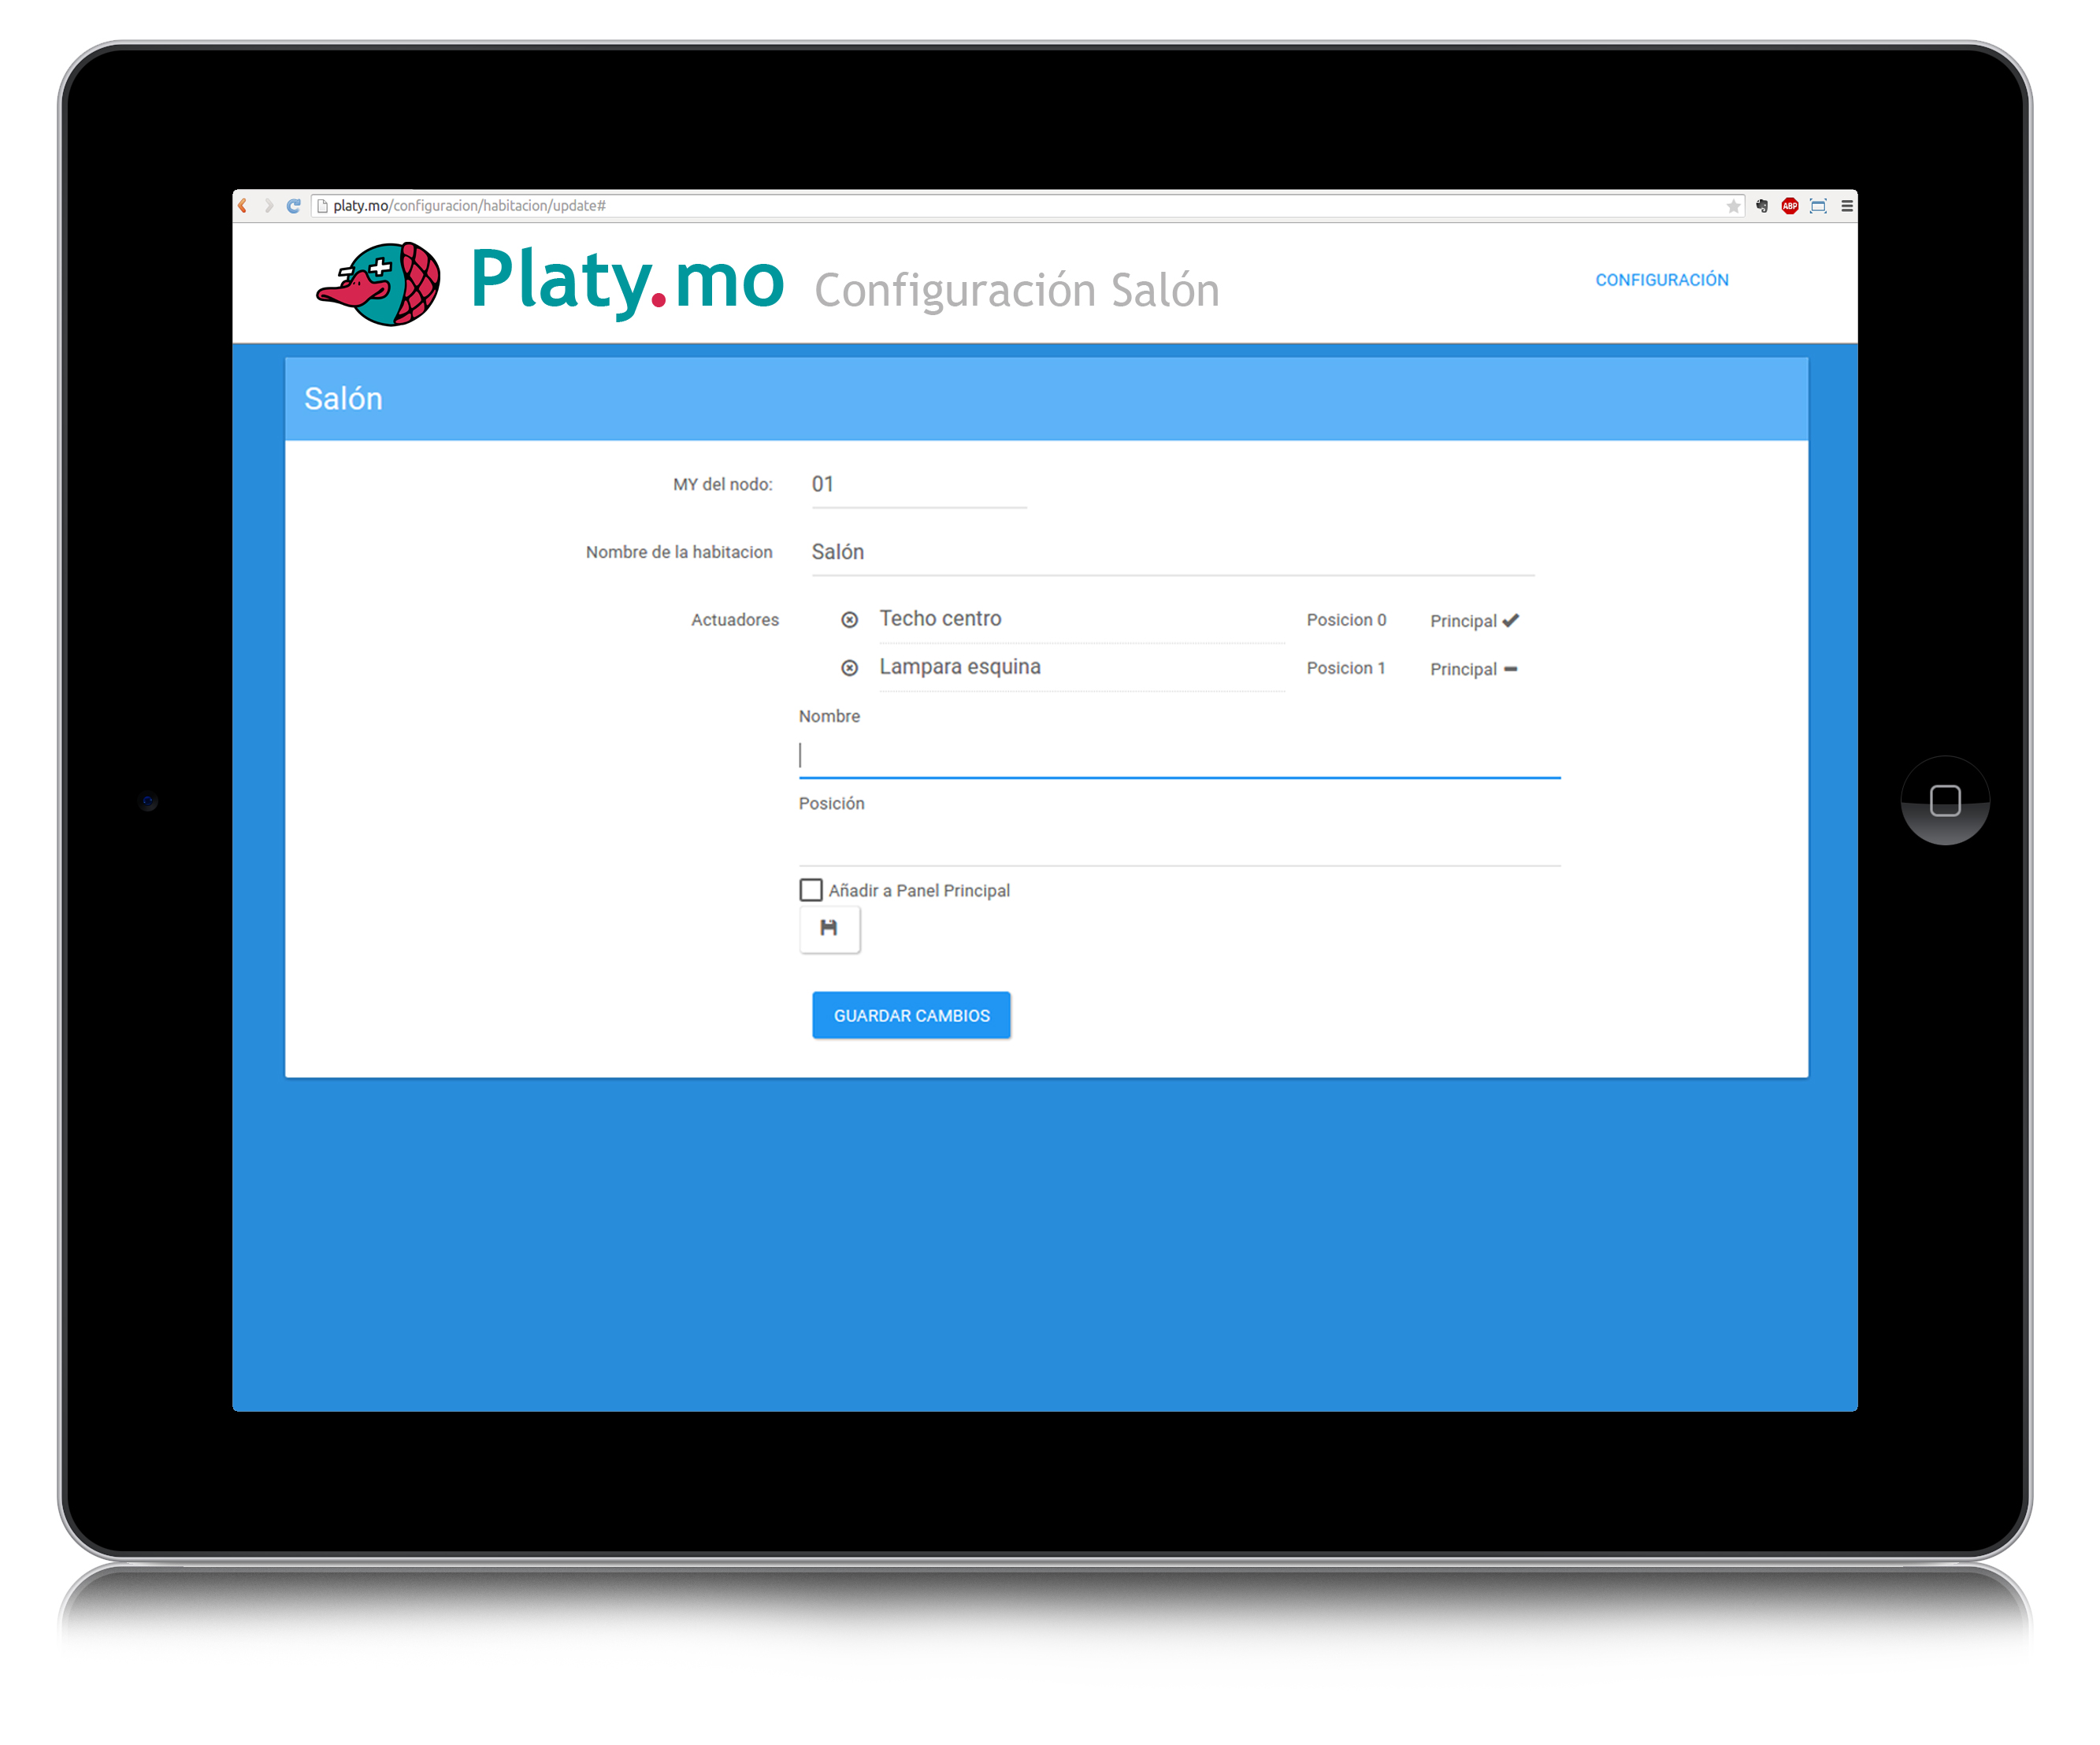
\includegraphics[width=0.95\textwidth]{imagenes/conf_hab.jpg}
            \caption{Formulario habitación}
            \label{fig:form_hab}
        \end{figure}
        
     Los actuadores se añaden de uno en uno. Una vez rellenados los campos correspondientes, se pulsa en el botón <<disquete>>, entonces los campos del actuador desaparecen, para mostrarse en la lista de los actuadores ya añadidos. Si quisiéramos añadir otro, pulsamos en el botón <<+>> y se creará otro juego vacío de campos para un actuador nuevo.
     
     En la lista de actuadores podemos ver los datos relativos a cada uno, y un enlace a la izquierda de cada uno para borrarlos.
     
          
     En el formulario para las escenas, introduciremos un nombre para ésta, y la configuración de luces que queramos, figura \ref{fig:form_esc}
    
    \begin{figure}[h!]
        \centering
        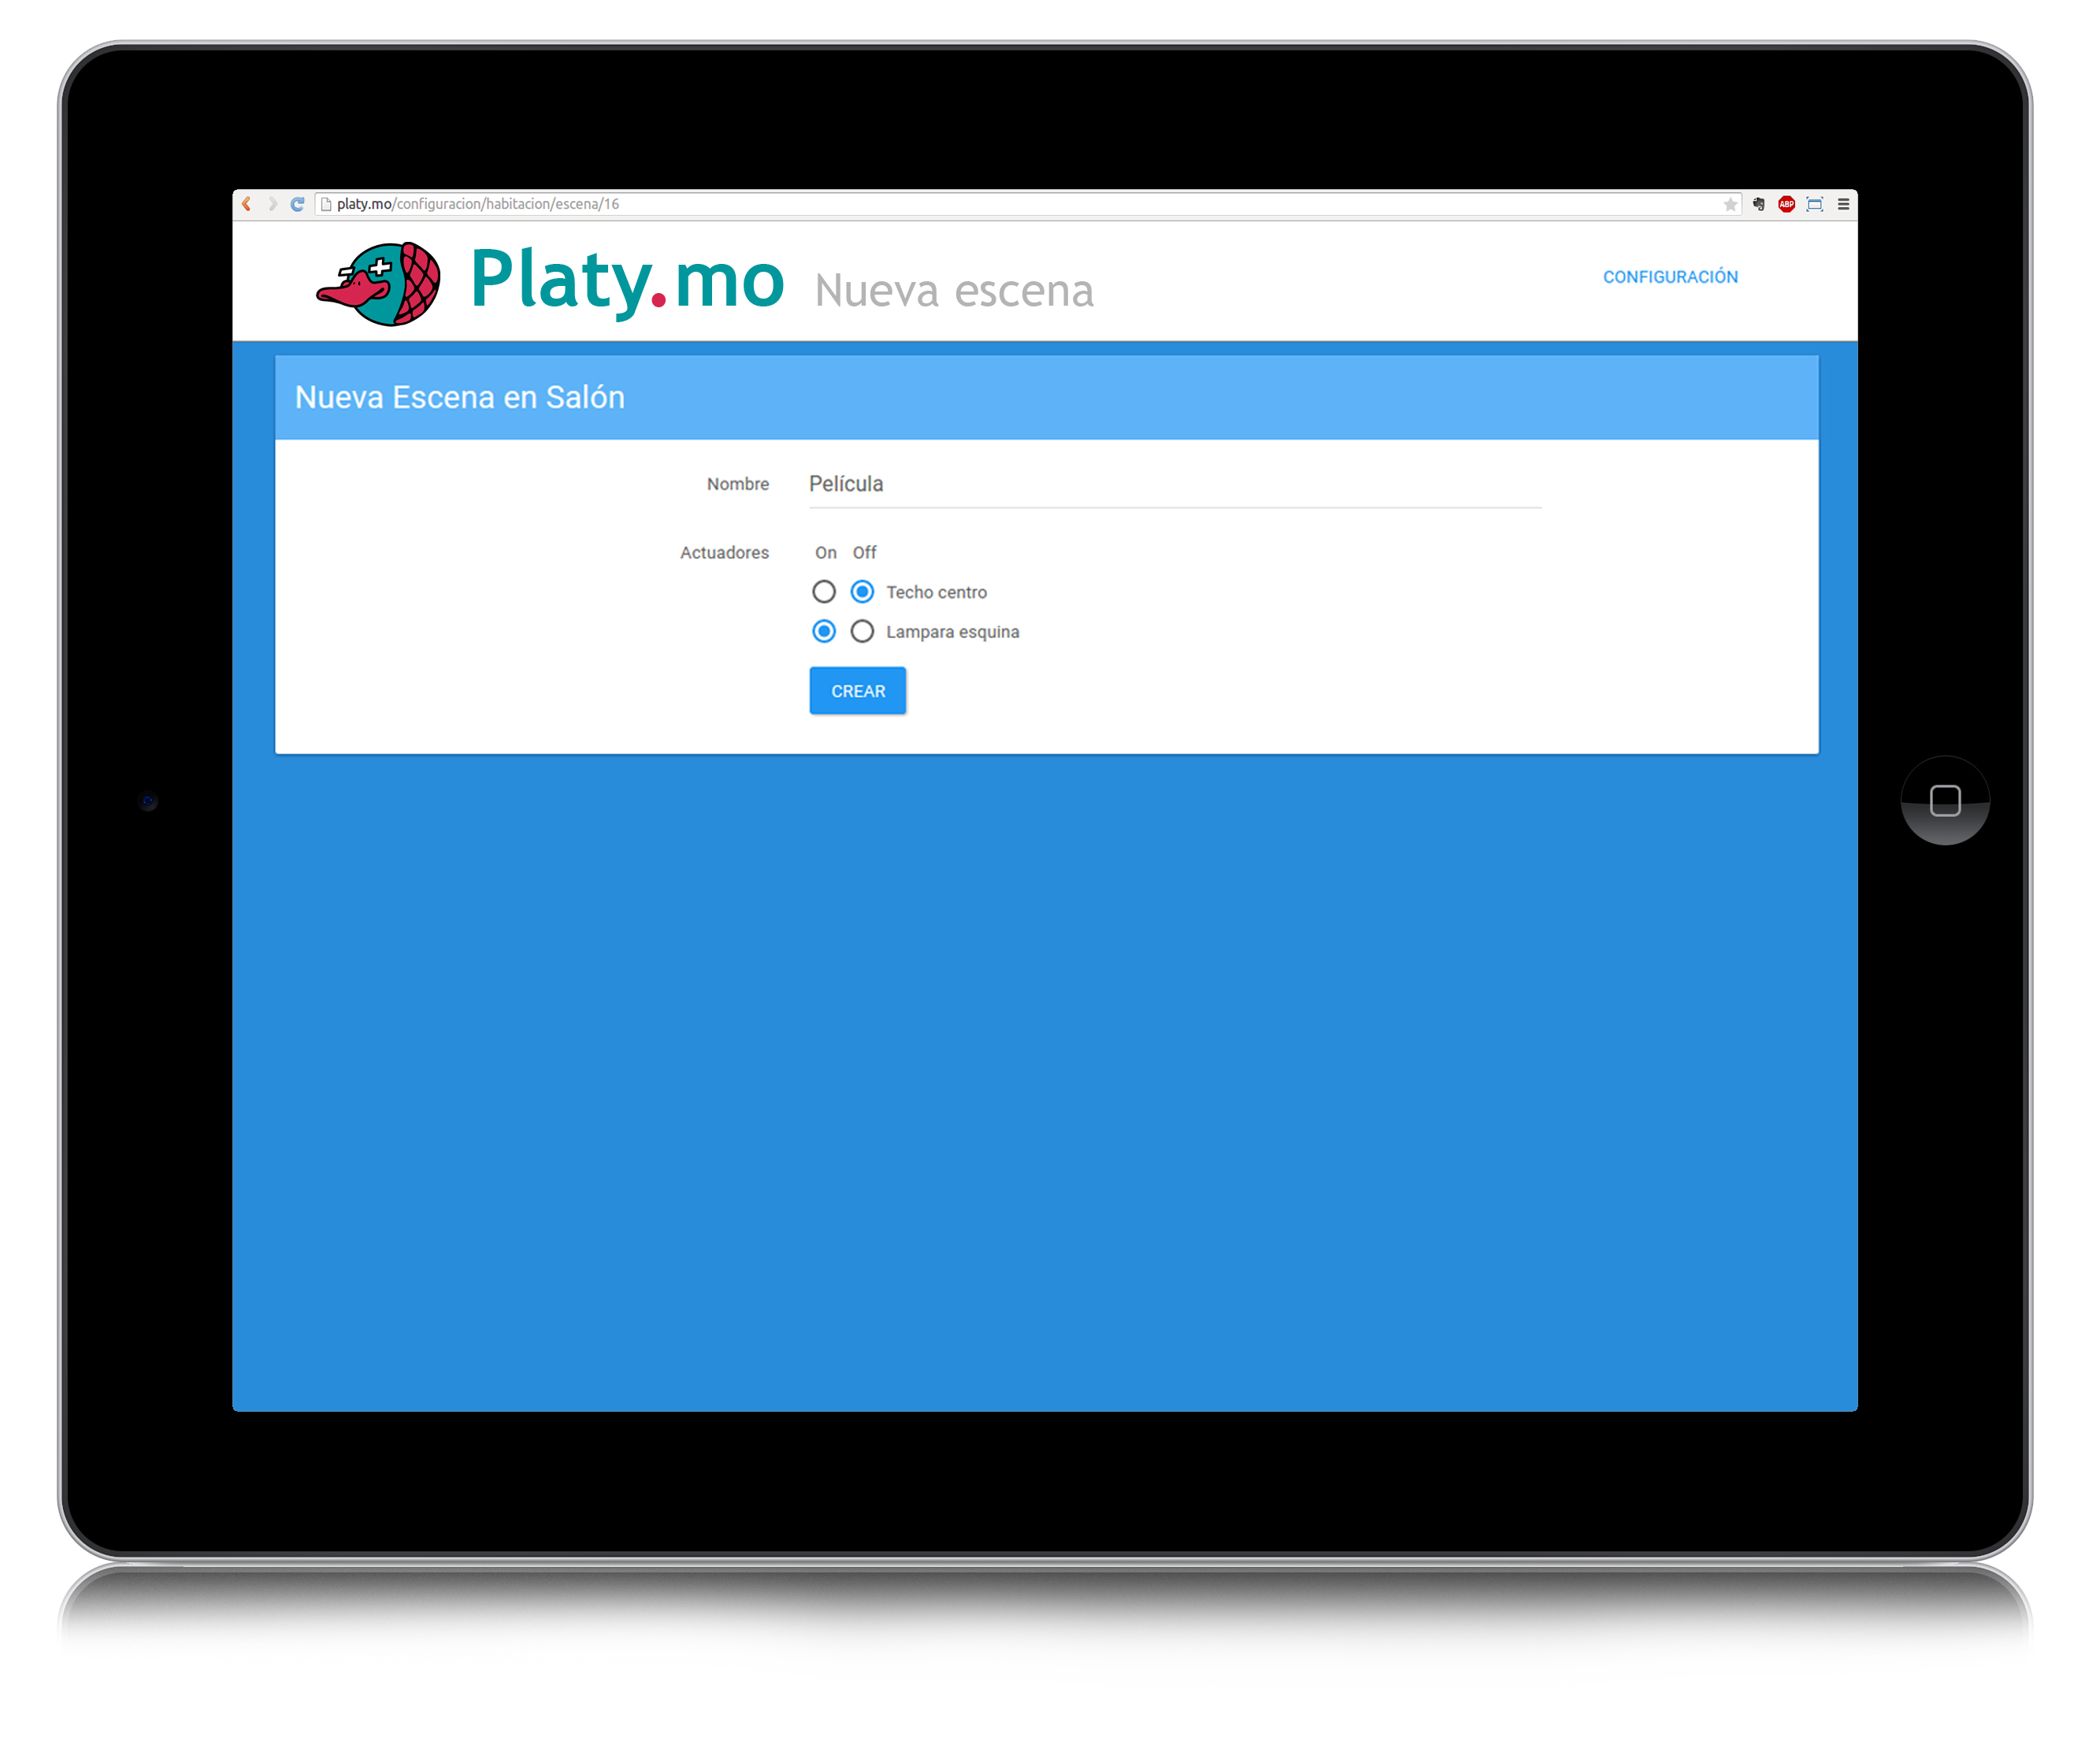
\includegraphics[width=0.95\textwidth]{imagenes/conf_esc.jpg}
        \caption{Formulario escena}
        \label{fig:form_esc}
    \end{figure}
    
    Por último, en el formulario para las acciones programadas veremos campos para: el nombre de la acción, el actuador que se programa, los días de la semana que queramos q se active, la hora, y si queremos que se encienda o apague.
    
    \begin{figure}[h!]
        \centering
        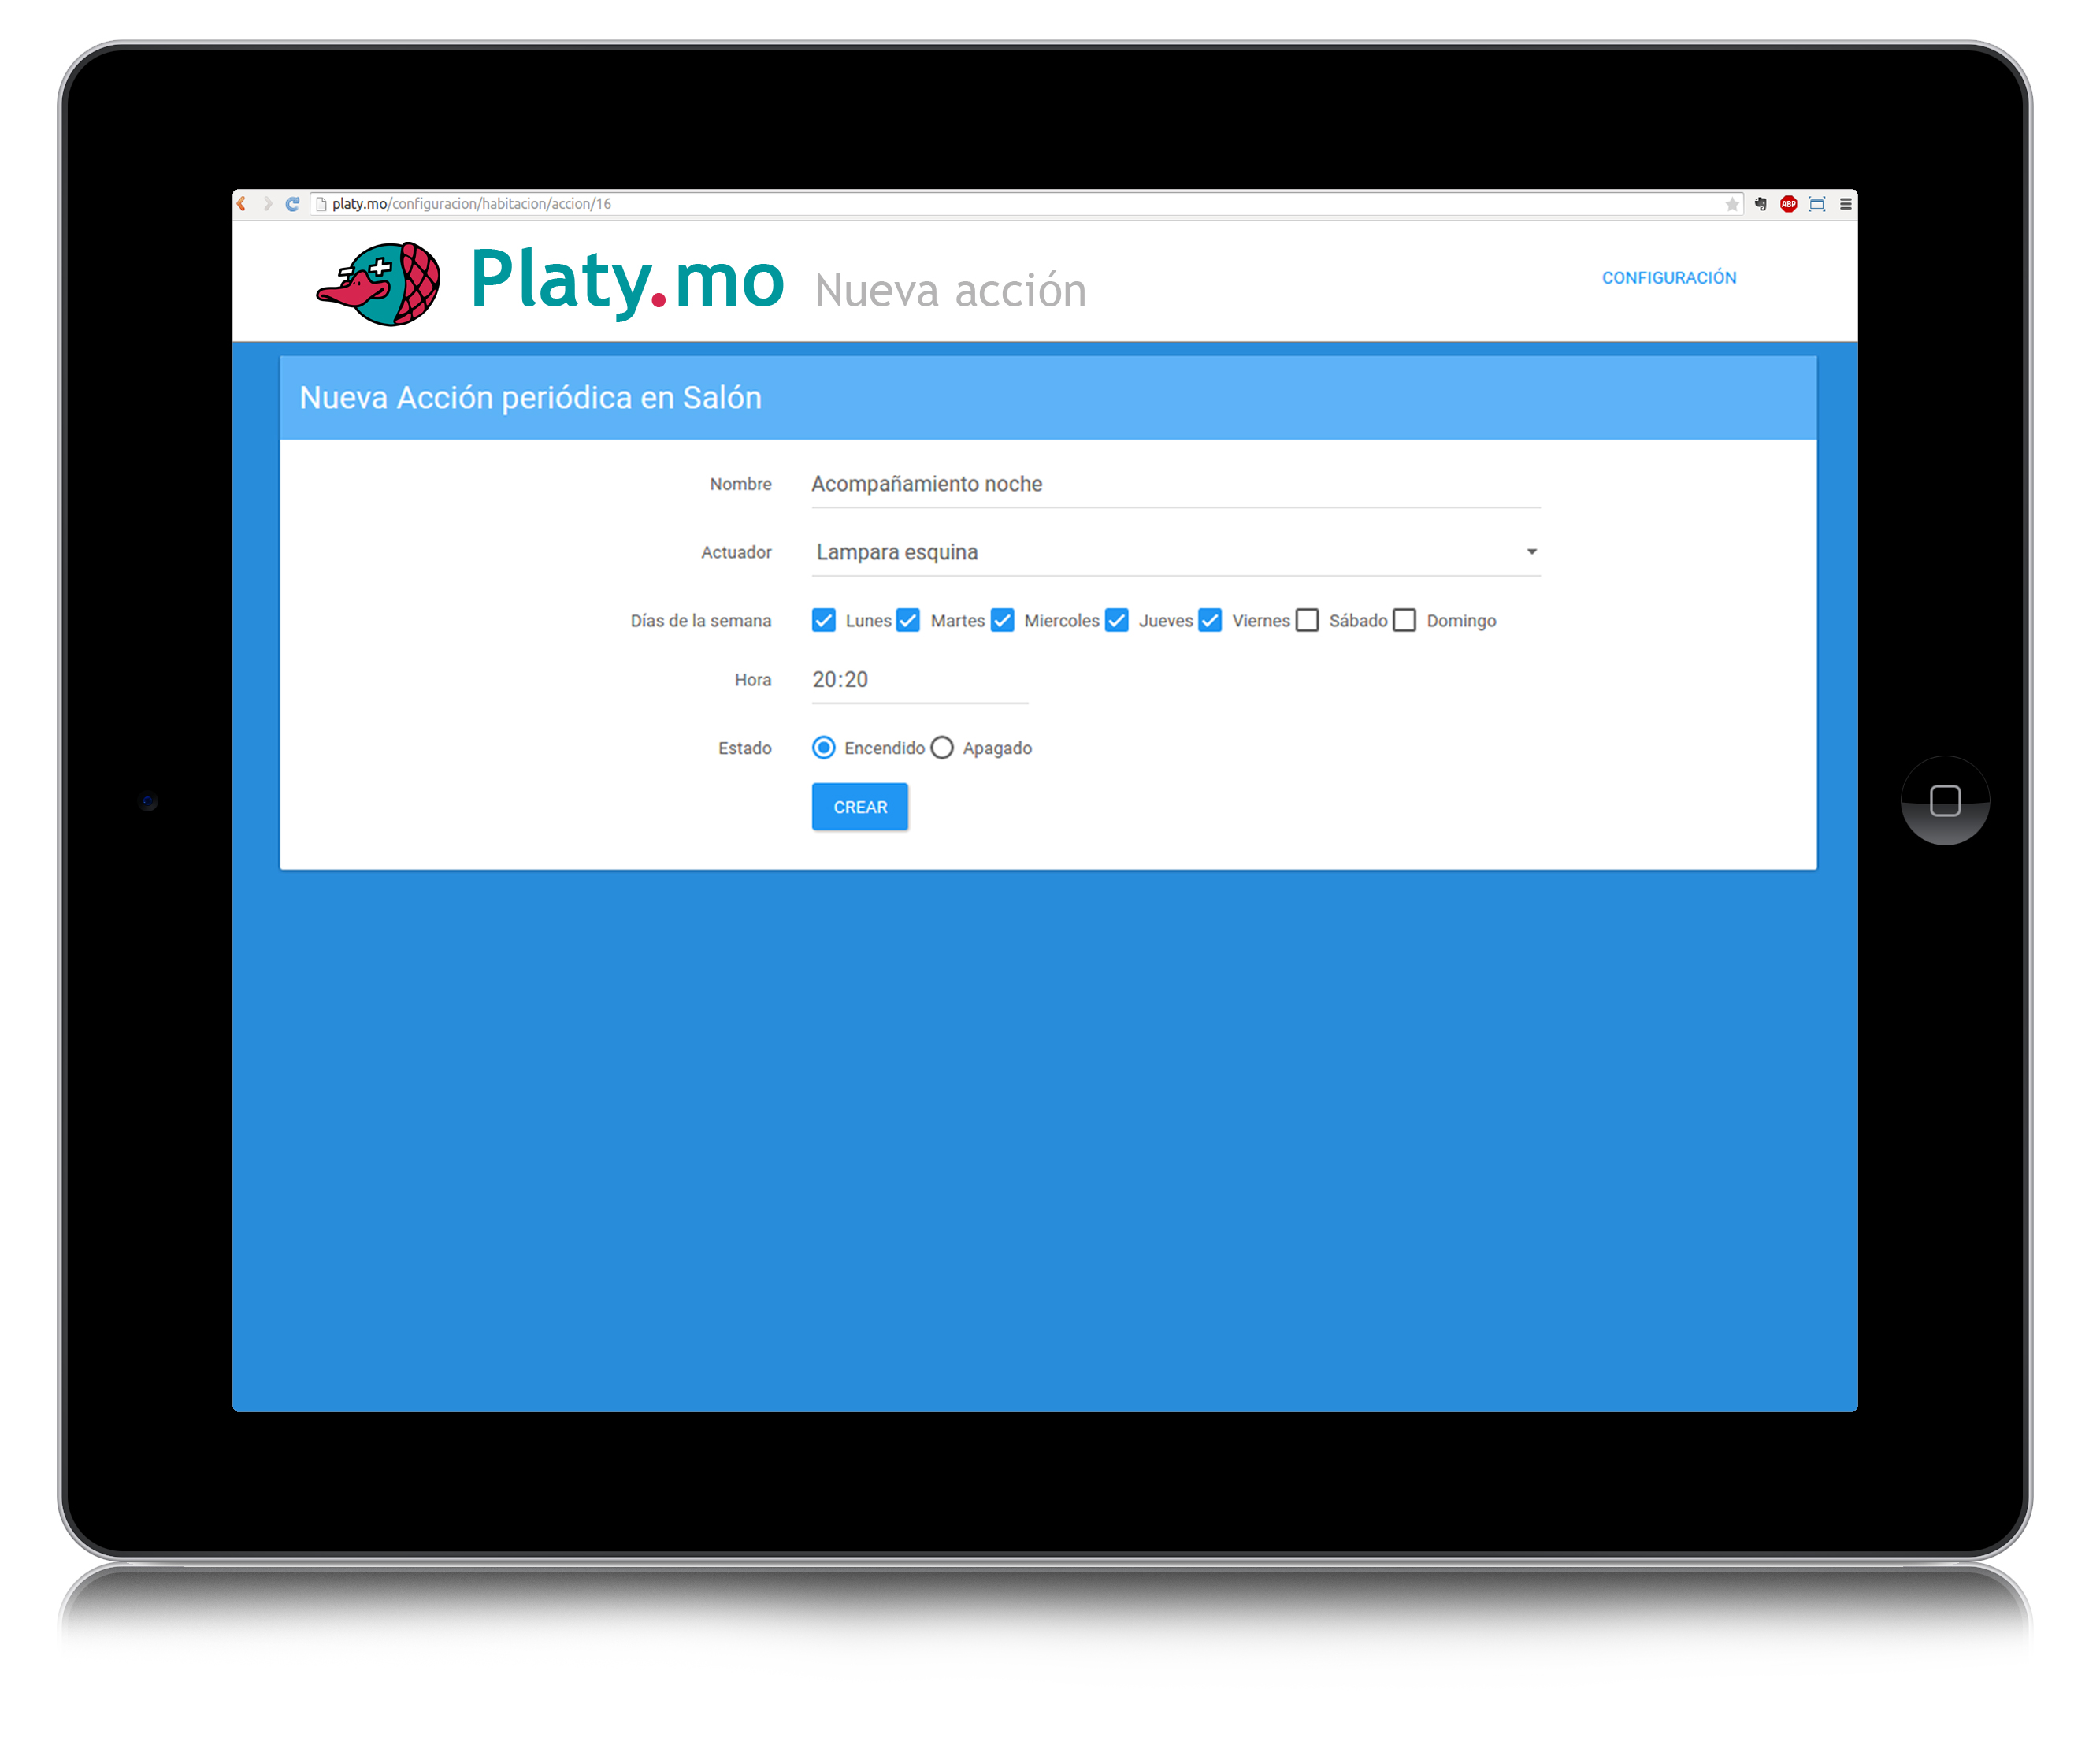
\includegraphics[width=0.95\textwidth]{imagenes/conf_accion.jpg}
        \caption{Formulario acción programada}
        \label{fig:form_acc}
    \end{figure}
    
    
    
  Para la gestión de todas las vistas y formularios, hemos creado diversos controladores.
    
    \begin{description}
        \item[HabitacionController] Actuadores y nodos.
        \item[EscenaController] Escenas.
        \item[AccionController] Acciones programadas.
    \end{description}
    
    El funcionamiento es similar para los tres controladores. Se crean 5 métodos, \lstinline|create()| y \lstinline|edit()| muestran los formularios, con \lstinline|store()| y \lstinline|update()| se procesan, y \lstinline|delete()| elimina el objeto en cuestión.
    
    Para mostrar el ciclo de funcionamiento, tomaremos como ejemplo el <<EscenaController>>.
    
    Al igual que antes, todo empieza con las rutas. En este caso tenemos:
    
    \begin{lstlisting}
Route::get('configuracion/habitacion/escena/{hab_id}', 
                    'EscenaController@create');

Route::post('configuracion/escena/store', 
                    'EscenaController@store');

Route::get('configuracion/escena/{id}',
                     'EscenaController@edit');

Route::post('configuracion/escena/update', 
                    'EscenaController@update');

Route::get('configuracion/escena/delete/{id}', 
                    'EscenaController@delete');
    
    \end{lstlisting}
    
    La primera de ellas, <</configuracion/habitacion/escena/\{hab\_id\}>>, renderiza el formulario para la creación de una escena nueva, en la habitación cuyo id sea <<hab\_id>>. El método encargado es \lstinline|create()|.
    
\begin{lstlisting}
public function create($hab_id){

    $habitacion = Nodo::find($hab_id);
    $actuadores = $habitacion->actuadores()->get();
    
    return view('config.escena')
        ->with(array('habitacion' => $habitacion,
                     'actuadores' => $actuadores,
                     'title' => 'Nueva escena'));
}
\end{lstlisting}
   
   El formulario creado, enviará la información recavada a <</configuracion/escena/store>>, según su ruta, se llamará al método \lstinline|store()|.
   
   \begin{lstlisting}
public function store(EscStoreFormRequest $request){

    $nodo = Nodo::find($request->get('hab_id'));
    
    $escena = new Escena;
    $escena->nombre = $request->get('nombre');
    
    $nodo->escenas()->save($escena);
    
    foreach ($nodo->actuadores()->get() 
                            as $actuador) {
        $estado = $request->get($actuador->id);
        $escena->actuadores()->
                attach($actuador->id, 
                      ['estado' => $estado]);
    }
  
    Session::flash('msg', 'Escena creada');
    return redirect('configuracion');
}
   \end{lstlisting}
   
   Aquí, podemos ver una de las características más útiles de Laravel, el sistema de validación. La variable que se introduce en la declaración del método es de una clase creada por nosotros <<EscStoreFormRequest>>, que hereda de la clase <<Request>>. Al introducir nuestra clase en la declaración, Laravel intercepta la petición, y antes de pasarla al método, le aplica las reglas de validación que incluyamos en nuestra clase. 
   
   Si no pasase la validación, Laravel automáticamente vuelve al formulario con los datos introducidos, y los mensajes de error pertinentes. Nunca llegaría al método \lstinline|store()|.
   
   \begin{lstlisting}
class EscStoreFormRequest extends Request {
    public function rules()
    {
        $rules = array(
        'nombre' => 'required|string|max:50'
        );
    
        return $rules;
    }
    
    public function messages(){
    
        return [
        'required' => 'El campo :attribute 
                    es obligatorio.',
        
        'string'=>'Solo se permiten caracteres 
              alfanumericos en el campo :attribute.',
                
        'max:50'=>'El campo :attribute puede tener 
                como maximo 50 caracteres.'
        ];
    }

}
    \end{lstlisting}
   
   Con la función \lstinline|rules()| se especifican las reglas de validación, y en \lstinline|messages()| se personalizan los mensajes de error.
   
   Si pasa la validación, entra en el método \lstinline|store()|. Creamos una escena nueva, se rellena y se guarda en  la base de datos.
   
   Otra característica de Laravel que podemos ver aquí, es la facilidad con la que se maneja la base de datos. En las escenas, al guardar una, también tenemos que guardar la configuración de los actuadores. Esto se realiza sobre una tabla pivote, en la que guardamos los id de ambas entidades junto con el valor que debe tomar el actuador. Lo que en principio puede ser una consulta más compleja, en Laravel simplemente llamamos a la función \lstinline|attach()|, esta función se encarga de todo por nosotros.
   
   Para la edición, procedemos de la misma forma. Con \lstinline|edit()| extraemos los datos y renderizamos el formulario. Más tarde, en \lstinline|update()|, tras pasar la validación, recuperamos la escena, modificamos los valores y guardamos.
   
   \begin{lstlisting}
public function edit($id){

   $escena = Escena::find($id);
   
   $habitacion = Nodo::find($escena->nodo()->
               first()->id);
   $actuadores = $habitacion->actuadores()->get();
   
   $query = DB::table('actuador_escena')
           ->where('escena_id', $escena->id)->get();
           
   $act_estado = array();
   $i = 0;
   foreach ($actuadores as $actuador) {
       $act_estado[$i] = array();
       $act_estado[$i]['id_actuador'] = $actuador->id;
       $act_estado[$i]['nombre'] = $actuador->nombre;
   
       foreach ($query as $row) {
   
           if($actuador->id == $row->actuador_id){
            $act_estado[$i]['estado'] = $row->estado;
           }
       }
       $i++;
   }





    return view('config.escenaEdit')
            ->with(array('habitacion' => $habitacion,
                'act_estado' => $act_estado,
                'escena' => $escena,
                'title' => $escena->nombre));
}


public function update(EscStoreFormRequest $request){

    $escena = Escena::find($request->get('esc_id'));
    $escena->nombre = $request->get('nombre');
    $escena->save();
    
    $data_sync = array();
    
    foreach (Nodo::find($escena->nodo_id)
                ->actuadores()->get() as $actuador) {
                
        $data_sync[$actuador->id] = 
          ['estado' => $request->get($actuador->id)];
    }
    
    $escena->actuadores()->sync($data_sync);
    
    Session::flash('msg', 'Escena modificada.');
    return redirect('configuracion');

}
\end{lstlisting}

En el método update hay que resaltar el uso de la función \lstinline|sync()|. Esta función sirve para sincronizar tablas pivote. Recibe un array con los id de una de las entidades implicadas, y actúa sobre la tabla para que solo contenga a estos id, ya sea borrando filas o añadiendo.

En nuestro caso, recibe un array con los id de los actuadores y el valor de estos, con lo que al final, la tabla queda actualizada con los nuevos datos.



\begin{lstlisting}



public function delete($id){

    $escena = Escena::find($id);
    $escena->delete();

    Session::flash('msg', 'Escena borrada.');
    return redirect('configuracion');
}
   \end{lstlisting}
   
   Para terminar, queda la acción de borrar escenas. Gracias a Laravel y su ORM, es muy sencillo. Traemos de la base de datos el objeto a borrar, y llamamos a su función \lstinline|delete()|.
   
   
   
    
    
    
    
    
    
    
  
  
  
  
  
  
  
 
 









